%! TEX program = lualatex

\documentclass[12pt]{ut-thesis}
%/========== Preamble ==========/%
\usepackage{adanstyle}

%---------- Bibliography Style ----------%
\usepackage[style=ieee,backend=biber]{biblatex}
\addbibresource{bib.bib}

%---------- Ut-Thesis Recommendations ----------%
%% List only down to subsections in the table of contents;
%% 0=chapter, 1=section, 2=subsection, 3=subsubsection, etc.
\setcounter{tocdepth}{2}

%% Make each page fill up the entire page.
\flushbottom

%/========== /Preamble ==========/%

%/========== Main Document ==========/%
\begin{document}

%---------- Preliminary Pages -----------%
\begin{preliminary}

% Generate the title page
%! TEX root = main.tex

%/========== Title Page Info ==========/%
\title{Energy injection for mechanical systems through the method of Virtual Nonholonomic Constraints}
\author{Adan Moran-MacDonald }
\degree{Master of Applied Science}
\department{Electrical and Computer Engineering}
\gradyear{2020}
\date{\today}

\maketitle
%/========== Title Page Info ==========/%

% vim: set ts=4 sw=4 sts=0 et ffs=unix :


%% There should be NOTHING between the title page and abstract.
%% However, if your document is two-sided and you want the abstract
%% _not_ to appear on the back of the title page, then uncomment the
%% following line.
\cleardoublepage

% Generate the abstract page, with line spacing adjusted according to SGS
% guidelines
%! TEX root = main.tex

%/========== Abstract ==========/%
%% (At most 150 words for M.Sc. or 350 words for Ph.D.)
\begin{abstract}
   This thesis develops a theoretical foundation for the framework of virtual
   nonholonomic constraints, which are relations between the generalized
   coordinates and generalized momenta of a mechanical system that can be
   enforced via feedback control.
   The theory is applied towards energy injection for two standard underactuated
   systems: the variable-length pendulum and the acrobot. 
   Virtual nonholonomic constraints are designed for each system by examining
   human motion, and energy injection properties of these constraints are proven
   rigorously.
   The acrobot constraint is tested on a real-world acrobot, demonstrating
   highly effective energy-injection properties and robustness to a variety of
   external disturbances.
\end{abstract}

%/========== /Abstract ==========/%
% vim: set tw=80 ts=4 sw=4 sts=0 et ffs=unix :


%% Anything placed between the abstract and table of contents will
%% appear on a separate page since the abstract ends with \newpage and
%% the table of contents starts with \clearpage.  Use \cleardoublepage
%% for anything that you want to appear on a right-hand page.

%% This generates the 'dedication' page, which will appear on a right-hand page
\cleardoublepage
%! TEX root = main.tex

\begin{dedication}
	\textbf{TODO}: Fill in the dedication
\end{dedication}
% vim: set ts=3 sw=3 sts=0 et ffs=unix :


%% The `dedication' and `acknowledgements' sections do not create new
%% pages so we need to separate them
\newpage  % separate pages for dedication and acknowledgements

%% This generates the "acknowledgements" section
%! TEX root = main.tex

%/========== Acknowledgements ==========/%

\begin{acknowledgements}
	\textbf{TODO}: Fill in the acknowledgements
\end{acknowledgements}

%/========== /Acknowledgements ==========/%
% vim: set ts=3 sw=3 sts=0 et ffs=unix :


%% This generates the Table of Contents (on a separate page).
\tableofcontents

%% This generates the List of Tables (on a separate page), if needed
%% (uncomment to have it appear in the document).
%\listoftables

%% This generates the List of Figures (on a separate page), if needed
%% (uncomment to have it appear in the document).
%\listoffigures

%% You can add commands here to generate any other material that belongs
%% in the head matter (for example, List of Plates, Index of Symbols, or
%% List of Appendices).

% TODO: Index of Symbols and Notation
%! TEX root = main.tex

%/========== Symbols ==========/%

% Set the heading so it appears in the Table of Contents
\addcontentsline{toc}{chapter}{List of Symbols}
\chapter*{List of Symbols}

% Define a table for the symbols using the booktabs convention
\noindent
\begin{table}[h!]
\resizebox{\textwidth}{!}{%
\centering
\begin{tabular}{ll}
   \toprule
   Symbol & Definition \\
   \midrule
   \(\R^n\) & Real numbers in \(n\) dimensions. \\
   \(\Rt{T}\) & Real numbers modulo \(T > 0\), with \(\Rt{\infty} = \R\). \\
   \(\mathbb{S}^1\) & The unit circle, equivalent to \(\Rt{2\pi}\). \\
   \(\R^{n \times m}\) & The space of real-valued matrices with \(n\) rows and \(m\) columns. \\
   \(\Id{n}\) & The \(n \times n\) identity matrix. \\
   \(\Zmat{n \times m}\) & The \(n \times m\) matrix of all zeros. \\
   \([M]_{i,j}\) & The value of row \(i\), column \(j\) for the matrix \(M\). \\
   \(\dot{x}\) & Derivative of \(x(t,y)\) with respect to time \(t\). \\
   \(x'\) & Derivative of \(x(t,y)\) with respect to a non-time input \(y\). \\
   \(\mathcal{Q}\) & The configuration manifold of a mechanical system. \\
   \(q_u\) & Unactuated coordinates. \\
   \(q_a\) & Actuated coordinates. \\
   \(p_u\) & Conjugate of momentum to \(q_u\). \\
   \(p_a\) & Conjugate of momentum to \(q_a\). \\
   \bottomrule
\end{tabular}

}% resizebox
\end{table}

%/========== /Symbols ==========/%
% vim: set ts=3 sw=3 sts=0 et ffs=unix :


%% End of the preliminary sections: reset page style and numbering.
\end{preliminary}

%---------- Main Content ----------%
TEST CITATIONS:

\cite{constrained_hamiltonian_systems}
\cite{control_giant_two_link_gymnastic_robot}
\cite{dynamical_servo_acrobot_vc}
\cite{dynamic_vhcs_stabilize_closed_orbits}
\cite{energy_pumping_robotic_swinging}
\cite{hamiltonian_nonholonomic_systems}
\cite{hamiltonization_of_nh_systems}
\cite{how_to_pump_a_swing}
\cite{hybrid_zero_dynamics_bipedal_nhvcs}
\cite{integrating_factors}
\cite{lagrangian_structure_reduced_dynamics_vhcs} 
\cite{multiple_lyapunov_functions}
\cite{multiple_lyapunov_functions_switched_systems}
\cite{nonholonomic_dynamics}
\cite{pendulum_length_giant_gymnastics}
\cite{pumping_swing_standing_squatting}
\cite{swingup_acrobot_pendulum}
\cite{swingup_giant_acrobot}
\cite{vhcs_for_el_systems}
\cite{vlp_energy_shaping}
\cite{xingbo_thesis}
\cite{khalil_nonlinear}
\cite{greenwood_dynamics}
\cite{landau_mechanics}
\cite{ida_pbc_underactuation_one}
\cite{ida_pbc_acrobot_example}
\cite{vhc_robotic_walking}
\cite{vhc_stable_walking}
\cite{vhc_snake}
\cite{vhc_bicycle}
\cite{vhc_helicopter}
\cite{vnhc_human_robot_cooperation}
\cite{psd_based_vnhc_redundant_manipulator}
\cite{haptic_vnhc}
\cite{vnhc_time_delay_teleop}
\cite{nhvc_dynamic_walking}
\cite{nhvc_incline_walking}
\cite{output_nhvc_bipedal_control}
\cite{dynamics_periodic_vlp}
\cite{oscillation_suppression_vlp}
\cite{vlp_tuned_mass_damper}

% When using external files, we use \input instead of \include because \input
% allows you to nest the inclusion. This way, we can separate the .tikz files
% for our images and still input them into the code.

% Introduce the thesis
%! TEX root = main.tex

%/========== Introduction ==========/%

\chapter{Introduction}

The Estonian sport of ``Kiiking" (Figure \ref{fig:kiiking}) is the adult
equivalent of a child playing on a standing swing, though here
an athlete attempts to make a giant solid steel swing gain momentum.
Naturally, the kiiker begins by pushing off the ground and proceeds to alternate
between standing and squatting. 
This allows them to swing higher and faster over time, until they have reached
their express goal of spinning at high speed around the bar.

\begin{figure}[h]
    \centering
    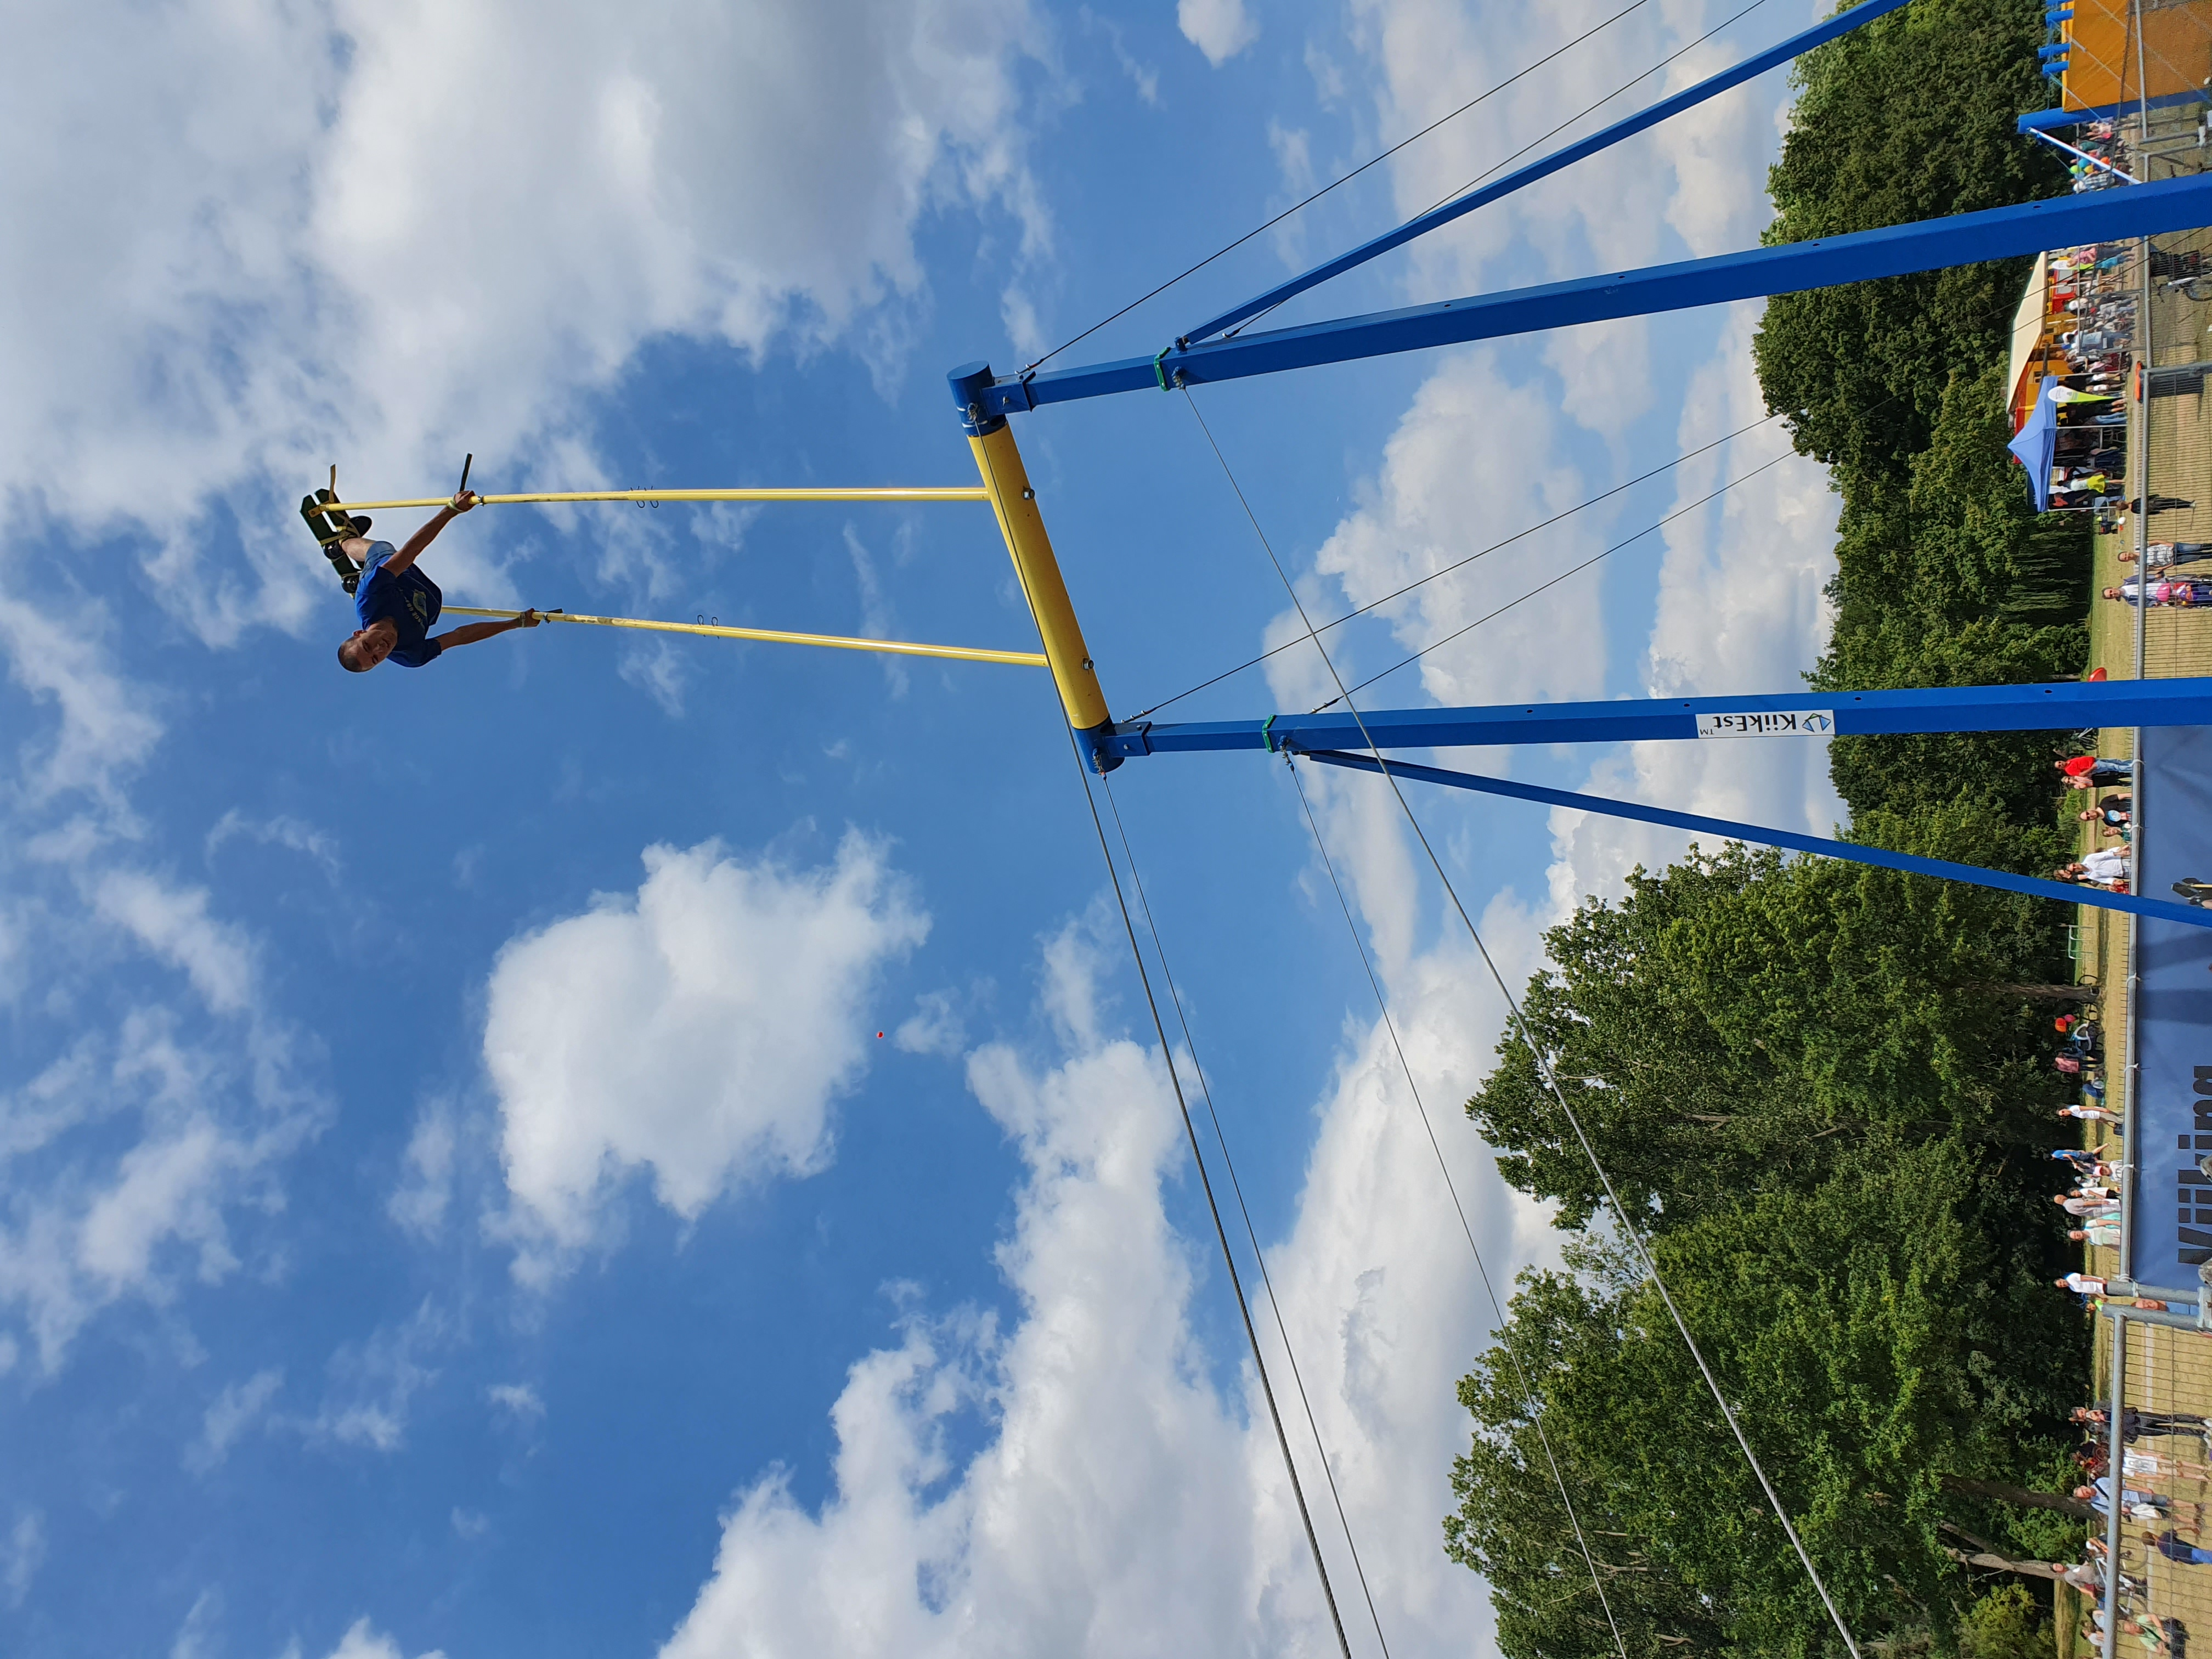
\includegraphics[width=0.6\textwidth,angle=270]{images/kiiking.jpg}
    \caption{Kiiking, which translates to ``swing", involves a person standing
        and squatting on a giant swing until they are rotating around the bar.
    Image taken from \cite{kiiking-img}.}
    \label{fig:kiiking}
\end{figure}

Now imagine that the kiiker is a robot, and their creator is teaching them to
swing like a human.
If the roboticist had studied classical control theory, they would plot 
a kiiker's squat depth as a trajectory over time and tell the robot to
synchronize with this trajectory.
In an ideal world, this technique would work perfectly; unfortunately, it is
also entirely unnatural. 
After all, humans on swings do not have an internal stopwatch telling them when
to squat.
Rather, they adjust how much they bend their knees based on the current angle of
the swing along with their direction of motion.
This position-velocity adjustment allows humans to correct for external
disturbances (like strong winds or enthusiastic swing pushers). 
Figure \ref{fig:swing-pos-vel} shows this adjustment process:
a person will squat when they reach the peak of their swing, and
stand when they reach the fastest point at the bottom
\cite{pumping_swing_standing_squatting}.
Even if the robot could perfectly track a time-based trajectory, an external
disturbance may affect where squatting and standing occurs to the point that
the swing actually slows down.

\begin{figure}
    \centering
    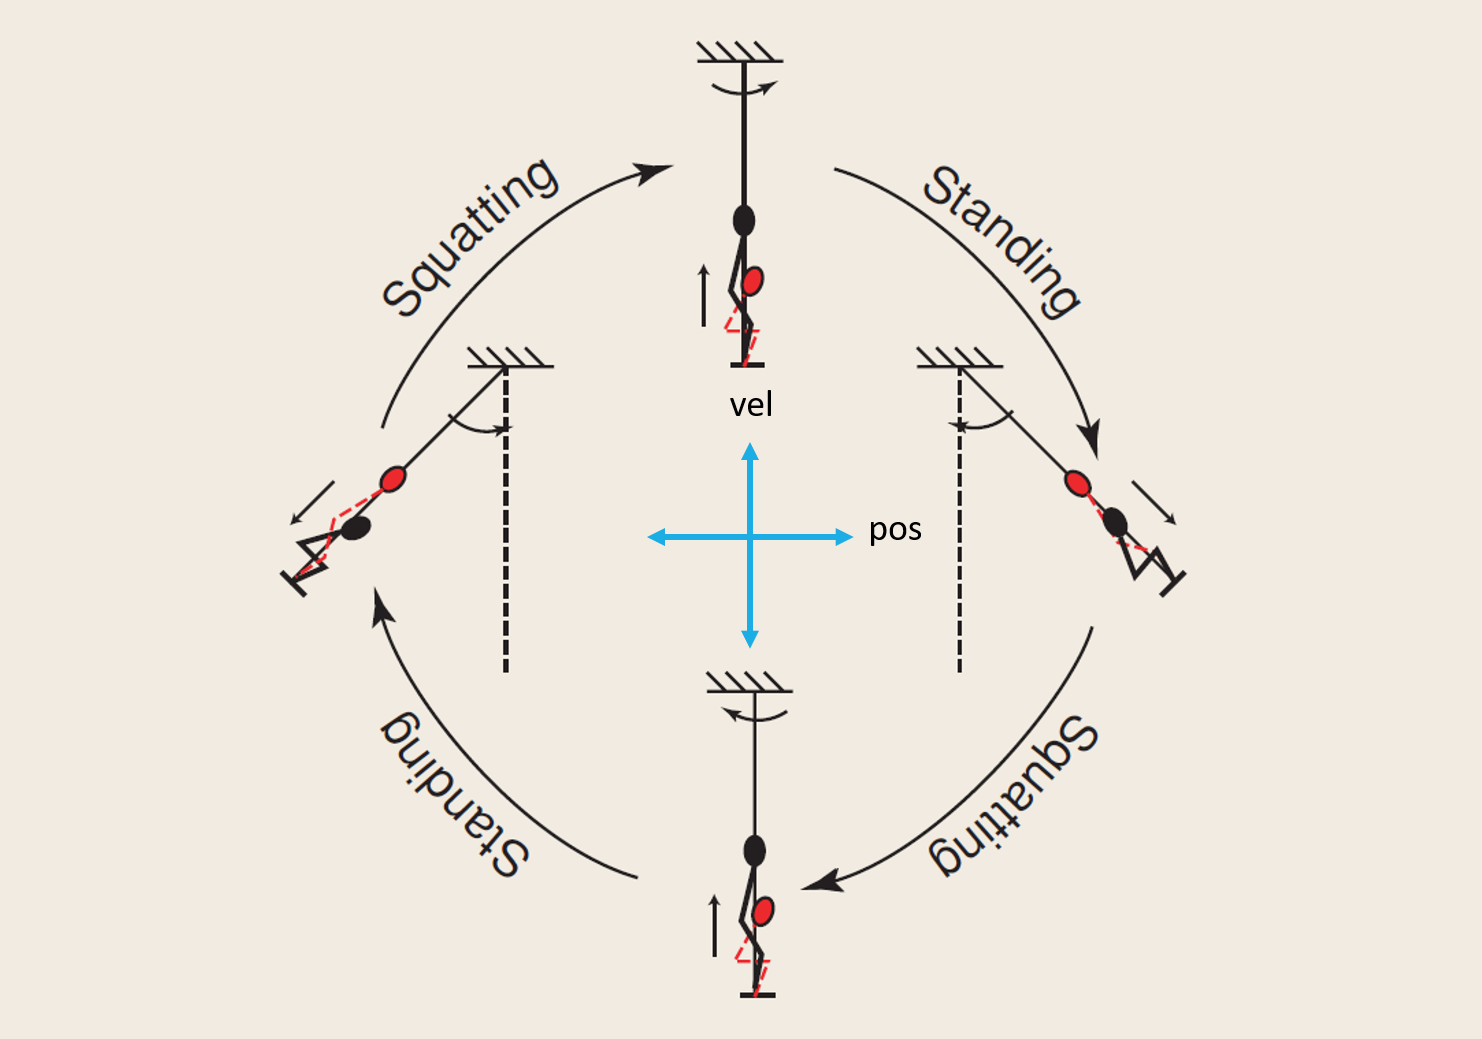
\includegraphics[width=0.75\textwidth]{images/swing_pos_vel.png}
    \caption{A person on a standing swing will stand at the bottom of the swing
        arc, and squat at the top. Figure modified from
        \cite{pumping_swing_standing_squatting}.}
    \label{fig:swing-pos-vel}
\end{figure}

To fix this issue, a clever roboticist might use \textit{virtual holonomic
constraints}, which are controllers that track a function of position rather
than time \cite{vhcs_for_el_systems}.
Sadly, this still fails since one needs velocity to determine when they
have reached the peak of their swing.
In other words, the robot needs to move according to a function of both position
and velocity if it has any hope of behaving like a real person.
These position-velocity controllers are known as 
\textit{virtual nonholonomic constraints}, and they are the focus of this
thesis.

Our goal throughout this thesis is to prove that virtual
nonholonomic constraints can increase a robot's momentum through a
process known as \textit{energy injection}.
We will use two benchmark robotic systems to build intuition and test
our theory.
The first system is the variable-length pendulum, which models a person
on a swing.
The second is the acrobot, an actuated double pendulum which models a gymnast
hanging on a horizontal bar.
For each of these examples, we will create virtual nonholonomic
constraints which model human motion and will rigorously prove that these
constraints inject energy. 

\section{Literature Review}
Let us review some of the existing research on energy injection and virtual
nonholonomic constraints.

Energy injection for mechanical systems is often performed by passivity-based
control and energy shaping --- one views the robot and its inputs as energy
transformations which are moulded to enforce desired behaviour.
Much of the theoretical work in this field has been performed by Ortega, van der
Schaft, and others (see for example \cite{ida_pbc_underactuation_one,
ida_pbc_acrobot_example,energy_shaping_revisited}).
Energy shaping has been applied to both the variable-length
pendulum \cite{vlp_energy_shaping} and the acrobot
\cite{swingup_acrobot_energy,swingup_giant_acrobot}.
This technique is useful and widely applicable, but it does not
produce the structured human-like motion we wish to generate using virtual
nonholonomic constraints.

The modern concept of virtual nonholonomic constraints was described by
\citet{nhvc_dynamic_walking} in 2015, though there are references to more
primitive versions going back as early as the the year 2000
\cite{vnhc_human_robot_cooperation}.
Virtual nonholonomic constraints have been of most notable use in
bipedal locomotion \cite{nhvc_incline_walking,output_nhvc_bipedal_control},
where they have shown marked improvements in the robustness of walking gaits
when compared to previous control technqiues.
They have also been used for error-reduction in time-delayed teleoperation
\cite{vnhc_time_delay_teleop} and in the field of human-robot interaction
\cite{psd_based_vnhc_redundant_manipulator,haptic_vnhc}.
All these research areas use different formulations of virtual nonholonomic constraints;
\citet{hybrid_zero_dynamics_bipedal_nhvcs} have derived the so-called
``constrained dynamics" for hybrid mechanical systems under virtual nonholonomic
constraints, but to the best of our knowledge no one has attempted to generalize
the concept to abstract mechanical systems.

Many of the contributions in this thesis are extensions of concepts from the
field of virtual holonomic constraints. 
Of note is the framework devised by Mohammadi, Maggiore, and
Consolini, among others
\cite{vhcs_for_el_systems,dynamic_vhcs_stabilize_closed_orbits,lagrangian_structure_reduced_dynamics_vhcs,xingbo_thesis}.

\section{Statement of Contributions}
Here are the contributions of this thesis.
\begin{itemize}[label={}]
   \item \textbf{Chapter \ref{ch:vnhcs}} The development of the framework of
      virtual nonholonomic constraints.
      This includes the definition of simply actuated mechanical systems, virtual
      nonholonomic constraints, regular constraints, and energy injection.
      Theorem \ref{thm:vnhc-regularity} yields a computational characterization
      of regularity, while Theorem \ref{thm:zero-dynamics} explicitly finds the
      constrained dynamics for a certain class of systems.
   \item \textbf{Chapter \ref{ch:vlp}} An application of virtual nonholonomic
      constraints to the variable-length pendulum, based on a pumping technique
      used by children on standing swings.
      The chapter culminates in Theorem \ref{thm:vlp-energy-stabilization},
      which guarantees that a certain class of VNHCs will inject energy into
      this system.
   \item \textbf{Chapter \ref{ch:acrobot}} An application of virtual
      nonholonomic constraints to the acrobot, based on the motion performed by
      human gymnasts.
      The chapter ends with Theorem \ref{thm:acrobot-energy-stabilization},
      which proves that the constraint we design does in fact inject energy into
      the acrobot.
\end{itemize}

\section{Organization of the Thesis}
The thesis is laid out as follows: 
in Chapter \ref{ch:vnhcs} we cover the requisite background on analytical 
mechanics, after which we develop the main theory of virtual nonholonomic
constraints;
in Chapter \ref{ch:vlp} we reformulate a time-optimal energy-injection strategy
for the variable-length pendulum as a virtual nonholonomic constraint, and
prove that the pendulum will gain enough energy to rotate around the bar with
arbitrary speed;
and in Chapter \ref{ch:acrobot} we find a virtual nonholonomic constraint 
which enables the acrobot to kick its legs like a gymnast until it
performs backflips on a horizontal bar.
Finally, we show experimental results on a physical acrobot which confirm
that the theory works in the real world.

%/========== /Introduction ==========/%
% vim: set tw=80 ts=4 sw=4 sts=0 et ffs=unix :


% Develop the formulation of VNHCs
%! TEX root = main.tex

%/========== Virtual Nonholonomic Constraints ==========/%

\chapter{Development of Virtual Nonholonomic Constraints}\label{ch:vnhcs}
% TODO: Brief introduction before preliminaries

\section{Preliminaries on Analytical Mechanics}
A mechanical system can be represented by \(N\) point masses where each point
represents the center of mass of a physical body, along with \(r\)
\textit{equations of constraint} (EOC) which model the physical restrictions
between these masses.
The position of each point mass is described using three cartesian coordinates (one
for each spatial axis), so the system as a whole can be described by a vector in
\(\R^{3N}\) with \(r\) EOC. 
The dynamics of the system are computed by deriving the \(3N\)
\textit{equations of motion} (EOM) produced by Newton's second law \(F = m a\).
While this technique works for simple systems, it is tedius and becomes
impossible to apply to complex mechanical systems where the forces are not
explicitly known. 

Rather than modeling a mechanical system by cartesian positions and constraints,
it is often feasible to represent the position of the system using \(n\)
independent scalar-valued variables \(q_1,\ldots,q_n\) called 
\textit{generalized coordinates}, where \(n = 3N - r\) is the number of
\textit{degrees of freedom} (DOF) of the system \cite{greenwood_dynamics}. For
instance, Figure \ref{fig:barbell} shows a barbell on a \(2D\)-plane which can
rotate freely on that plane. 
The barbell has \(n = 3\) DOF, so it can be described by three
independent generalized coordinates with no equations of constraint.

\begin{figure}
   \centering
   \begin{subfigure}[]{0.75\textwidth}
      \includestandalone[width=\textwidth]{images/newtonian_barbell}
      \caption{The Newtonian representation of the barbell 
      requires all six cartesian positions and the corresponding EOC.}
   \end{subfigure}
   \begin{subfigure}[]{0.75\textwidth}
      \includestandalone[width=\textwidth]{images/gc_barbell}
      \caption{One possible set of three generalized coordinates is
       \((x_0,y_0,\theta)\), which represent the position of the 
       center of the bar and the angle of the barbell in the \(xy\)-plane.}
   \end{subfigure}
   \caption{A mechanical system with \(N = 2\) point masses at \(a = (x_1,y_1,z_1)\)
       and \(b = (x_2,y_2,z_2)\), separated by a bar of length \(c\). 
       There are \(r = 3\) EOC given by \(\norm{a - b} = c\), \(z_1 = 0\),
       and \(z_2 = 0\). This system has \(n = 3\) degrees of freedom.}
   \label{fig:barbell}
\end{figure}

For the robotic systems of interest in this thesis, we assume that
each generalized coordinate \(q_i\) represents either the distance or the angle
between two parts of the system.
Mathematically, each \(q_i\) takes values in \(\Rt{T_i}\), where
\(T_i = \infty\) if \(q_i\) represents a length or \(T_i = 2\pi\) if \(q_i\)
represents an angle.
It is convention to collect the coordinates into a \textit{configuration} 
\(q = (q_1,\ldots,q_n) \in \mathcal{Q}\) 
where the \textit{configuration manifold} \(\mathcal{Q}\) of the system is a
so-called \textit{generalized cylinder}:
\[
    \mathcal{Q} = \Rt{T_1} \times \cdot \times \Rt{T_n}
    .
\] 
The derivative \(\dot{q} = (\dot{q}_1,\ldots,\dot{q}_n)\) of a configuration
is called a \textit{generalized velocity} of the system. For arbitrary systems,
the space of allowable velocities depends on the current configuration of the
system.  However, since \(\mathcal{Q}\) is a generalized cylinder, we find that 
\(\dot{q} \in \R^n\).
The combined vector \((q,\dot{q}) \in \mathcal{Q}\times\R^n\) is called a 
\textit{state} of the system.

The field of analytical mechanics provides a computational method for finding
the EOM of a system in generalized coordinates. The two most common analytical
methods for modelling robotic systems are \textit{Lagrangian} and
\textit{Hamiltonian} mechanics.

% ---------- Lagrangian Mechanics ---------- % 
\subsection{Lagrangian Mechanics}\label{sec:lagrangian-mechanics}

Lagrangian mechanics uses the kinetic energy \(T(q,\dot{q})\) and potential
energy \(P(q)\) of the system to define the Lagrangian 
\(\mathcal{L} : \mathcal{Q}\times\R^n \rightarrow \R\) defined by
(\ref{eqn:lagrangian-general}) \cite{greenwood_dynamics}:
\begin{equation}\label{eqn:lagrangian-general}
    \mathcal{L}(q,\dot{q}) = T(q,\dot{q}) - P(q)
    .
\end{equation}
When the mechanical system is actuated, the EOM are described by \(n\) second-order
ordinary differential equations (ODEs) obtained from the \textit{Euler-Lagrange
equations} (\ref{eqn:el-eqns-general}) with \textit{generalized input forces} 
\(\tau \in \R^k\)
\begin{equation}\label{eqn:el-eqns-general}
    \diff{}{t}\left\{ \pdiff{\mathcal{L}}{\dot{q}_i} \right\}
    - \pdiff{\mathcal{L}}{q_i} = B_i\tpose(q) \tau
    .
\end{equation}
The vector \(B_i\tpose: \mathcal{Q} \rightarrow \R^{1\times k}\) describes how
the input forces shape the dynamics of \(q_i\).
The matrix  \(B: \mathcal{Q} \rightarrow \R^{n \times k}\) with
\[
    B(q) = \begin{bmatrix}
        - & B_1\tpose(q) & - \\
          & \vdots & \\
        - & B_n\tpose(q) & - \\
    \end{bmatrix}
    ,
\]
is called the \textit{input matrix} for the system.
If \(k < n\), we say the system is \textit{underactuated} with degree of
underactuation \((n - k)\).

Many actuated mechanical systems have quadratic kinetic energies, so that the
Lagrangian can be written explicitly as
\begin{equation}\label{eqn:lagrangian}
    \mathcal{L}(q,\dot{q}) = \frac{1}{2} \dot{q}\tpose D(q) \dot{q} - P(q)
    ,
\end{equation}
where the \textit{inertia matrix} \(D: \mathcal{Q} \rightarrow \R^{n\times n}\) 
is a symmetric, positive definite matrix for all \(q \in \mathcal{Q}\) and the
potential function \(P : \mathcal{Q} \rightarrow \R\) is smooth. 
%If this is the case, the Euler-Lagrange equations reduce to (\ref{eqn:el-eqns}),
%\begin{equation}\label{eqn:el-eqns}
%    D(q)\ddot{q} + C(q,\dot{q})\dot{q} + \nabla P(q) = B(q)\tau
%\end{equation}
%where the \textit{Coriolis matrix} \(C(q,\dot{q})\) is of the form
%\[
%    [C]_{i,j} = \frac{1}{2}\sum\limits_{k = 1}^n 
%    \left(\pdiff{D_{i,j}}{q_k}  +
%     \pdiff{D_{i,k}}{q_j} -
%     \pdiff{D_{k,j}}{q_i}\right)\dot{q}_k
%\]

% ---------- Hamiltonian Mechanics ---------- %
\subsection{Hamiltonian Mechanics}
Hamiltonian mechanics converts the \(n\) second-order ODEs generated by
Lagrangian mechanics into an equivalent set of \(2n\) first-order ODEs.

To do this, we first define the \textit{conjugate of momentum \(p_i\) to \(q_i\)} by
\begin{equation}\label{eqn:p-i}
    p_i(q,\dot{q}) := \pdiff{\mathcal{L}}{\dot{q}_i}(q,\dot{q})
    .
\end{equation}
To ease notation, we write \(p = (p_1, \ldots, p_n) \in \R^n\) and call
\(p\) the \textit{conjugate of momenta to \(q\)}.
Note that each \(p_i\) is a linear function of \(\dot{q}\), and one can typically
solve for \(\dot{q}(q,p)\) by inverting all the expressions from (\ref{eqn:p-i}).
The combined vector \((q,p) \in \mathcal{Q}\times\R^n\) is called a 
\textit{phase} of the system. 

The \textit{Hamiltonian} of the system in
\(\{q,p\}\) coordinates is the ``Legendre transform"
(\ref{eqn:hamiltonian-legendre}) of the Lagrangian \cite{landau_mechanics},
\begin{equation}\label{eqn:hamiltonian-legendre}
    \mathcal{H}(q,p) := p\tpose \dot{q}(q,p) - \mathcal{L}(q,\dot{q}(q,p))
    .
\end{equation}
The EOM in the Hamiltonian framework are the \(2n\)
first-order equations called \textit{Hamilton's equations}. They are given by
\begin{equation}\label{eqn:hamiltons-eqns}
    \begin{cases}
        \dot{q} = \nabla_p\mathcal{H} \\
        \dot{p} = -\nabla_q\mathcal{H} + B(q)\tau
        .
    \end{cases}
\end{equation}
Here, \(B(q) \in \R^{n\times k}\) is the same input matrix used by the
Lagrangian framework, with \(\tau \in \R^k\) the same vector of generalized
input forces.

If the kinetic energy of the system is quadratic as in (\ref{eqn:lagrangian}), 
the conjugate of momenta becomes \(p = D(q)\dot{q}\). Since \(D(q)\) is symmetric
and positive definite, it is invertible at each \(q \in \mathcal{Q}\).
The Legendre transform (\ref{eqn:hamiltonian-legendre}) can be explicitly
written as
\[
    \mathcal{H}(q,p) = p\tpose D\inv(q)p - \frac{1}{2}p\tpose D\inv(q) p + V(q)
    ,
\]
which reduces to (\ref{eqn:hamiltonian}). 
Finding the derivative of each conjugate of momentum yields
\[
    \dot{p}_i = -\frac{1}{2} p\tpose \nabla_{q_i}D\inv(q) p 
        - \pdiff{P}{q_i}(q) + B_i\tpose(q) \tau
    ,
\]
which can be collected into the vector form (\ref{eqn:hamiltonian-full-dynamics}) 
% TODO: Update Appendix info?
by using the matrix Kronecker product (see Appendix ???).
In sum, when the kinetic energy is quadratic the Hamiltonian system reduces to
\begin{align}\label{eqn:hamiltonian}
    \mathcal{H}(q,p) &= \frac{1}{2} p\tpose D^{-1}(q) p + P(q)
    , \\
     &\begin{cases}
        \dot{q} = D\inv(q)p \\
        \dot{p} = -\frac{1}{2} (\Id{n} \otimes p\tpose) \nabla_q D\inv(q) p
        - \nabla_q P(q) + B(q) \tau
        . \\
    \end{cases} \label{eqn:hamiltonian-full-dynamics}
\end{align}

Any set of coordinates \((q,p)\) which satisfy Hamilton's equations 
under the Hamiltonian \(\mathcal{H}\) are
said to be \textit{canonical coordinates} for the system. A change of
coordinates \((q,p) \rightarrow (Q,P)\) is a \textit{canonical
transformation} if \((Q,P)\) preserve the Hamiltonian structure; that is, if
they are canonical coordinates under the Hamiltonian
\(\mathcal{H}\left(q(Q,P), p(Q,P)\right)\).

\citet{landau_mechanics} provides a useful result for showing whether a given
change of coordinates \((q,p) \to (Q,P)\) is a canonical transformation.
\begin{defn}
    The \textit{Poisson bracket} between the functions \(f(q,p)\) and \(g(q,p)\)
    is defined as
    \begin{equation}\label{eqn:poisson-bracket}
        [f,g] := \sum \limits_{i=1}^n \pdiff{f}{p_i}\pdiff{g}{q_i} - 
            \pdiff{f}{q_i}\pdiff{g}{p_i}
        .
    \end{equation}
\end{defn}
\begin{thm}\label{thm:canonical-transformations}
    A change of coordinates 
    \((q,p) \to (Q,P)\) is a canonical transformation if
    \begin{align*}
        [Q_i, Q_j] &= 0
        , \\
        [P_i, P_j] &= 0
        , \\
        [P_i, Q_j] &= \delta_{i,j}
        , 
    \end{align*}
    for all \(i,j \in \n\).
\end{thm}
\begin{proof}
    See (45.10) in \cite{landau_mechanics}.
\end{proof}

Later in this chapter we will define a particular type of coordinate change.
The following Lemma allows us to prove it is a canonical transformation.

\begin{lemma}\label{lemma:linear-is-canonical}
    Let \(\mathcal{H}\) be a Hamiltonian system in canonical coordinates
    \((q,p)\).
    Let \(A \in \R^{n\times n}\) be an invertible matrix such that
    \(A\inv = A\tpose\).
    The change of coordinates \((q,p) \to (Q = Aq, P = Ap)\) is a canonical
    transformation.
\end{lemma}
\begin{proof}
    For any constant matrix \(A\), the transformation
    \((Q = Aq, P = Ap)\) satisfies
    \(\pdiff{Q_i}{p_m} = \pdiff{P_i}{q_m} = 0\) for all 
    \(i,m \in \n\).
    Hence, 
    \begin{align*}
        [Q_i,Q_j] &:= \sum\limits_{m = 1}^n \pdiff{Q_i}{p_m}\pdiff{Q_j}{q_m} - 
        \pdiff{Q_i}{q_m}\pdiff{Q_j}{p_m} = 0
        , \\
        [P_i,P_j] &:= \sum\limits_{m=1}^n \pdiff{P_i}{p_m}\pdiff{P_j}{q_m} -
        \pdiff{P_i}{q_m}\pdiff{P_j}{p_m} = 0
        .
    \end{align*}
    Note that \((A_i)\tpose (A\tpose)_j = (A_i)\tpose (A\inv)_j = \delta_{i,j}\). 
    Using this fact we see that the Poisson brackets between \(P_i\) and \(Q_j\)
    are given by
    \begin{align*}
        [P_i,Q_j] &= \sum\limits_{m=1}^n\pdiff{P_i}{p_m}\pdiff{Q_j}{q_m}
        - \pdiff{P_i}{q_m}\pdiff{Q_j}{p_m} \\
                  &= \sum\limits_{m=1}^n A_{i,m}A_{j,m} - 0 \\
                  &= \sum\limits_{m=1}^n A_{i,m}A\tpose_{m,j} \\
                  &= (A_i)\tpose (A\tpose)_j \\
                  &= \delta_{i,j}
        .
    \end{align*}
    Therefore, by Theorem \ref{thm:canonical-transformations}, the coordinate
    change \((Q = Aq, P = Ap)\) is a canonical transformation.
\end{proof}

\section{Simply Actuated Hamiltonian Systems}\label{sec:simply-actuated}
% Describe the change of coordinates to get into q_u/q_a mode and show
% that the actuator directly affects pa but not pu. Use M for simply actuated
% inertia, D for normal coordinates
Suppose we are given a Hamiltonian mechanical system (\ref{eqn:hamiltonian}).
Because \(\tau\) is transformed by the input matrix \(B(q)\) before
entering the EOM, it is not in general clear how any particular input force \(\tau_i\)
will affect the dynamics of the system. 
In this section, we define a new class of Hamiltonian systems where the effect
of the input forces is made obvious. This class of
systems will form the backbone for the rest of the theory developed in this
thesis.

\begin{defn}
    Let \(\mathcal{H}\) be an \(n\)-DOF Hamiltonian system 
    with \(k \leq n\) actuators. 
    A set of canonical coordinates \((q,p)\) for this system
    are said to be \textit{simply actuated coordinates} if the
    input matrix \(B(q) \in \R^{n \times k}\) is of the form
    \[
        B(q) = \simpleB    
        .
    \]
    The first \((n-k)\) coordinates, labelled \(q_u\), are called the
    \textit{unactuated coordinates}. The remaining \(k\) coordinates, labelled
    \(q_a\), are called the \textit{actuated coordinates}. When grouping them
    together, we will always put them in the order \((q_u, q_a)\) to fit with 
    the definition. 
    The corresponding \((p_u, p_a)\) are called the \textit{unactuated} and 
    \textit{actuated momenta}, respectively.
\end{defn}

Under the following assumptions on the input matrix, we will show that there is
a canonical transformation of (\ref{eqn:hamiltonian}) into simply actuated
coordinates.

\begin{assm}\label{assm:B-const}
    The input matrix \(B(q) \equiv B \in \R^{n\times k}\) is constant,
    full rank, and \(k < n\).
\end{assm}
\begin{assm}\label{assm:B-perp}
    There exists a matrix 
    \(B^\perp \in \R^{(n-k)\times n}\)
    which is right semi-orthogonal 
    \(\left(B^\perp(B^\perp)\tpose = \Id{(n-k)}\right)\)
    and which is a left-annihilator for \(B\). 
    That is, \(B^\perp B = \Zmat{(n-k) \times k}\).
\end{assm}

Assumption \ref{assm:B-perp} requires the rows of \(B^\perp\) to be unit vectors
that are mutually orthogonal. 
In the case that \(k = (n-1)\), the existence of any left annihilator 
\(A^0 \in \R^{1\times n}\) implies the left annihilator 
\(B^\perp := A^0/\norm{A^0}\) will satisfy Assumption \ref{assm:B-perp}.

\begin{lemma}\label{lemma:B-orthogonal}
    Suppose Assumption \ref{assm:B-const} holds. Then
    there exist nonsingular matrices \(V,T \in \R^{k \times k}\) 
    so that the regular feedback transformation 
    \[
        \tau = V T \hat{\tau}
    \] 
    has a new input matrix \(\hat{B}\) for \(\hat{\tau}\) which is left
    semi-orthogonal.  
    That is, \(\hat{B}\tpose \hat{B} = \Id{k}\).
\end{lemma}
\begin{proof}
Since \(B\) is a constant matrix, 
it has a singular-value decomposition 
\(B = U \Sigma V\tpose\) where \(U^{-1} = U\tpose \in \R^{n \times n}\), 
\(V^{-1} = V\tpose \in \R^{k \times k}\), and \(\Sigma \in \R^{n \times k}\) is
defined by
\[
    \Sigma = \begin{bmatrix}
        \sigma_1 & 0 & \cdots & 0 \\
        0 & \sigma_2 & \cdots & 0 \\
        \vdots & & \ddots & \vdots \\
        0 & 0 & \cdots & \sigma_k \\
        - &   & \Zmat{(n-k)\times k} & -  \\
    \end{bmatrix}
    ,
\]
where \(\sigma_i \neq 0\) because \(B\) is full-rank \cite{calculating_svd}.
Defining \(T \in \R^{k \times k}\) by
\[
    T = \begin{bmatrix}
        \frac{1}{\sigma_1} & 0 & \cdots & 0 \\
        0 & \frac{1}{\sigma_2} & \cdots & 0 \\
    \vdots & & \ddots & \vdots \\
    0 & 0 & \cdots & \frac{1}{\sigma_k} \\
    \end{bmatrix}
    ,
\]
and defining the regular feedback transformation\(\tau = V T \hat{\tau}\), 
we get a new input matrix for \(\hat{\tau} \in \R^k\) given by 
\[
    \hat{B} = B V T = 
    U \begin{bmatrix}
        \Id{k} \\ \Zmat{(n-k)\times k}
    \end{bmatrix}
    ,
\]
which is still constant and full-rank. 
In particular, 
\(\hat{B}\tpose \hat{B} = T\tpose \Sigma\tpose \Sigma\tpose T = \Id{k}\).
\end{proof}

In light of Lemma \ref{lemma:B-orthogonal}, there is no loss of generality
making the following assumption.
\begin{assm}\label{assm:B-orthogonal}
    Assume that the input matrix \(B\) is
    left semi-orthogonal. 
\end{assm}

Let now \(\mathbf{B} \in \R^{n\times n}\) be the following matrix:
\[
    \mathbf{B} = 
    \begin{bmatrix}
        B^\perp \\
        B\tpose \\
    \end{bmatrix}
    .
\]
Since \(B^\perp\) is a left annihilator of \(B\) and both \(B^\perp\) and
\(B\tpose\) are right semi-orthogonal, it is easy to show that \(\mathbf{B}\) is
orthogonal:
\begin{proof}
\[
    \mathbf{B}\mathbf{B}\tpose = 
    \begin{bmatrix}
        B^\perp (B^\perp)\tpose & B^\perp B \\
        (B^\perp B)\tpose & B\tpose B
    \end{bmatrix} = \Id{n}
    .
\]
Hence, \(\mathbf{B}\) is invertible with \(\mathbf{B}\inv = \mathbf{B}\tpose\).
\end{proof}

The following theorem shows that \(\mathbf{B}\) provides a canonical
transformation into simply actuated coordinates, so that only the actuated momenta
are affected by the input forces.

\begin{thm}\label{thm:simply-actuated}
    Under Assumptions \ref{assm:B-const},\ref{assm:B-perp}, and
    \ref{assm:B-orthogonal}, the Hamiltonian system (\ref{eqn:hamiltonian})
    has simply actuated canonical coordinates 
    \(\{Q = \mathbf{B}q, P = \mathbf{B}p\}\). The resulting dynamics are 
    given by (\ref{eqn:simple-hamiltonian}),
    \begin{align}\label{eqn:simple-hamiltonian}
        \mathcal{H}(Q,P) &= 
        \frac{1}{2} P\tpose \Minv(Q) P + V(Q)
        , \\
       &\begin{cases}
            \dot{Q} = \Minv(Q)P \\
            \dot{P} = -\frac{1}{2} (\Id{n} \otimes P\tpose) \nabla_Q \Minv(Q) P
                - \nabla_Q V(Q) + \simpleB \tau
            ,
        \end{cases} \nonumber
    \end{align}
    where
    \begin{align*}
        \Minv(Q) &:= \mathbf{B}D^{-1}(\mathbf{B}\tpose Q)\mathbf{B}\tpose
        , \\
        V(Q) &:= P(\mathbf{B}\tpose Q)
        .
    \end{align*}
\end{thm}
\vspace{-4.5em} % For some reason not having this puts a large space before proof
\begin{proof}
    The change of coordinates \((Q = \mathbf{B}q, P = \mathbf{B}p)\)
    satisfies Lemma \ref{lemma:linear-is-canonical}, making it a canonical
    transformation.
    Furthermore, since \(\dot{P} = \mathbf{B}\dot{p}\), the new input matrix is
    given by 
    \[
        \mathbf{B}B = \begin{bmatrix}
            B^\perp B \\
            B\tpose B \\
        \end{bmatrix} = 
        \begin{bmatrix}
            \Zmat{(n-k)\times k} \\
            \Id{k}
        \end{bmatrix}
        ,
    \]
    which means \(\left(Q = (q_u,q_a), P = (p_u,p_a)\right)\) are simply
    actuated coordinates for \(\mathcal{H}\) as desired.
\end{proof}

\section{Virtual Nonholonomic Constraints}
% Motivation for VNHCs, they are an extension of VHCs, etc.
Let us imagine a child on a swing who wants to reach the largest height
possible. 
To begin, the child pushes off the ground to imbue the swing with small oscillations.
What allows them to increase the amplitude of these oscillations is the
appropriate extension and retraction of their feet.
If a roboticist were creating a machine to replicate this behaviour, they might
design a robot whose legs extend and retract at specific time intervals. 
At first glance, this technique should work perfectly because the leg motion
would synchronize with the swinging frequency, thereby injecting energy as
quickly as is physically possible.

Unfortunately, a deeper analysis reveals the flaw with this design.
Most children are not counting out the time in their head; rather, they observe
their current position and velocity and adjust their legs as required. 
For example, many children have an adult pushing the swing, or perhaps
they are swinging on a windy day. In either case, they adjust their leg
motion accordingly when presented with these external disturbances, without
keeping track of time. 
Hence, the standard control technique of tracking a function of time (known as
\textit{trajectory tracking}) does not truly replicate human behaviour.
Even if the robot's legs perfectly track a specified trajectory, 
an external disturbance will desynchronize the leg motion
with the swing - thereby stopping the amplitude-increasing effects.

%As has been observed in the field of mobile robotics, a trajectory tracking
%controller which has lagged behind due to a disturbance will do whatever is
%required to ``catch up" to the trajectory. 
%This can cause major safety issues, which is why many mobile roboticists prefer to
%design controllers which drive a vehicle along a gemoetric path in space rather than a
%trajectory in time.

%This path tracking approach has been extended to biologically-inspired robotics
%in a method known as \textit{virtual holonomic constraints} (VHCs).
Rather than tracking a trajectory over time, a more human-like behaviour 
is to force the robot's legs track a function of the swing's state. 
One recent control method known as \textit{virtual holonomic constraints} (VHCs)
uses the actuators to enforce a relation \(h(q) = 0\) of the configuration
\cite{vhcs_for_el_systems}. 
This method has provided incredible results in the development of 
walking robots \cite{vhc_robotic_walking, vhc_stable_walking}, 
vehicle motion \cite{vhc_bicycle, vhc_helicopter}, 
and has even been used to design a snake-like swimming robot
\cite{vhc_snake}.

The downside to VHCs is that they only depend on the configuration of a
mechanical system, and not its generalized velocity.
For the child on a swing, whether they extend or retract their legs
depends on their direction of motion. 
This inherently requires knowledge of their current velocity, which precludes
the usage of VHCs. 
A few authors have attempted to extend the theory of VHCs to enforce relations
\(h(q,\dot{q}) = 0\) of the full state to account for this drawback. 
Since these relations use actuators to restrict both the configuration and
velocity of a system, they are called virtual \textit{nonholonomic} constraints.
This idea has been used for human-robot interaction
\cite{vnhc_human_robot_cooperation,psd_based_vnhc_redundant_manipulator,haptic_vnhc},
error-reduction on time-delayed systems \cite{vnhc_time_delay_teleop},
and has shown marked improvements to the field of bipedal locomotion 
\cite{nhvc_dynamic_walking,
hybrid_zero_dynamics_bipedal_nhvcs,output_nhvc_bipedal_control}.
Most interestingly, this nonholonomic approach is more robust
than standard VHCs when applied to bipedal robotics \cite{nhvc_incline_walking}.
In particular, virtual nonholonomic constraints may be capable of injecting and
dissipating energy from a system in a robust manner, all while producing
realistic biological motion. This is what we aim to prove in this thesis.

Unlike the theory of VHCs, there does not appear to be a standard definition of
virtual nonholonomic constraints: 
all the applications listed above use their own definitions, which makes it
difficult to compare and generalize their work. 

This section will provide a standard characterization of virtual nonholonomic
constraints using Hamiltonian mechanics. 
The goal is to provide a consistent, rigorous foundation for designing
constraints on a general class of systems.

% Perform the full development of VNHCs, including its stabilizing
% controller.
\begin{defn}
    A \textit{virtual nonholonomic constraint} (VNHC) \textit{of order \(k\)} is a
    relation \(h(q,p) = 0\) where \(h : \mathcal{Q}\times\R^n \rightarrow \R^k\) is
    \(C^2\), \(\rank{\left[ dh_q,\, dh_p \right]} = k\) for all 
    \((q,p) \in h\inv(0)\), and there exists a feedback controller \(\tau(q,p)\)
    stabilizing the \textit{constraint manifold}
    \[
        \Gamma = \left\{(q,p) \mid h(q,p) = 0, dh_q \dot{q} + dh_p \dot{p} = 0\right\}
        .
    \]
\end{defn}

From the definition of VNHCs, one finds that the constraint manifold \(\Gamma\)
is a \(2(n-k)\)-dimensional surface inside \(\mathcal{Q} \times \R^n\). 
The next obvious question is the following: when does a feedback controller
stabilizing \(\Gamma\) exist?

One approach to answering this question is to
define the error term \(e = h(q,p)\). 
Finding \(\tau(q,p)\) driving \(e \to 0\) and \(\dot{e} \to 0\)
is sufficient for stabilizing \(\Gamma\). 
If \(\tau\) appears after only \(r_i \geq 0\) derivatives of \(e_i\), 
then that \(e_i\) is said to have \textit{relative degree} \(r_i\).
We would then say \(e\) has relative degree \(\{r_1,\ldots,r_k\}\).

One important note is that having relative degree \(1\) for any \(e_i\) means we
may not be able to stabilize \(\Gamma\); we can guarantee \(h(q,p) \to 0\) 
but not \(\dot{h}(q,p) = 0\). 
Requiring that \(e\) have relative degree \(\{2,\ldots,2\}\) is much more
useful, since it allows us to easily solve for a \(\tau\) which stabilizes
\(\Gamma\). 
This is a common requirementa in the VHC literature, so we will make use of it
here by defining a special type of VNHC that satisfies this property.

\begin{defn}
    A VNHC \(h(q,p) = 0\) of order \(k\) is \textit{regular} if the output 
    \(e = h(q,p)\) is of relative degree \(\{2,2.\ldots,2\}\) everywhere on the
    constraint manifold \(\Gamma\).
\end{defn}

The authors of
\cite{nhvc_dynamic_walking,hybrid_zero_dynamics_bipedal_nhvcs,nhvc_incline_walking}
observed that a relation which uses only the unactuated conjugate of momentum
cannot have \(\tau\) appearing after only one derivative. Of course,
they performed their research in Lagrangian form; we will be using
the Hamiltonian formulation from Chapter \ref{sec:simply-actuated}.
As a reminder, our system is described in \((q,p)\) coordinates with 
\(q = (q_u,q_a)\) and \(p = (p_u, p_a)\) and has the dynamics
\begin{align}\label{eqn:simply-actuated-hamiltonian}
    \mathcal{H}(q,p) &= p\tpose \Minv(q) p + V(q)
    , \\
    \label{eqn:simply-actuated-dynamics}
    &\begin{cases}
       \dot{q} = \Minv p \\
       \dot{p} = -\frac{1}{2} \pdmat - \nabla_q V(q) + \simpleB \tau 
       .\\
    \end{cases}
\end{align}

\begin{notation}
    We will write \(q_u \in \mathcal{Q}_u\), \(q_a \in \mathcal{Q}_a\) where
    \(\mathcal{Q}_u \times \mathcal{Q}_a = \mathcal{Q}\). 
    We also write
    \(p_u \in \mathcal{P}_u := \R^{n-k}\) and 
    \(p_a \in \mathcal{P}_a := \R^k\), so that 
    \(p \in \mathcal{P} := \mathcal{P}_u \times \mathcal{P}_a = \R^n\). 
    In this manner, the phase space of our system can be written as
    \(\mathcal{Q} \times \mathcal{P}\).
\end{notation}

\begin{thm}\label{thm:vnhc-regularity}
    A VNHC \(h(q,p) = 0\) of order \(k\) is regular if and only if \(dh_{p_a} = 0\) 
    and
    \[
        \rank{\left(dh_q \Minv(q) - 
          dh_{p_u} (\Id{n-k} \otimes p\tpose)\nabla_{q_u}\Minv(q) 
         \right)\simpleB} = k
         ,
    \]
    everywhere on the constraint manifold \(\Gamma\).
\end{thm}
\begin{proof}
    Let \(e = h(q,p) \in \R^k\). Then 
    \begin{align*}
        \dot{e} &= dh_q \dot{q} + dh_p \dot{p} \\
                &= dh_q \Minv(q)p +{}  \\
            & \begin{bmatrix} dh_{p_u} & dh_{p_a} \end{bmatrix}
        \left( -\frac{1}{2} \begin{bmatrix}
            (\Id{n-k} \otimes p\tpose) \nabla_{q_u}\Minv(q)p \\
            (\Id{k} \otimes p\tpose) \nabla_{q_a}\Minv(q)p
            \end{bmatrix} - \begin{bmatrix}
            \nabla_{q_u}V(q) \\
            \nabla_{q_a}V(q)
        \end{bmatrix} + \simpleB \tau\right)
        .
    \end{align*}
    If \(dh_{p_a} \neq \Zmat{k \times k}\) for some \((q,p)\) on \(\Gamma\), 
    then \(\tau\) appears in \(\dot{e}\) and the VNHC is not of relative degree
    \(\{2,2,\ldots,2\}\).
    Hence, we must have that \(dh_{p_a} = \Zmat{k \times k}\).
    Proceeding with this assumption, we now find that
    \(h : \mathcal{Q} \times \mathcal{P}_u \rightarrow \R^k\), which means that
    \[
        \dot{e} = dh_q \Minv(q)p - 
        dh_{p_u} \left(\frac{1}{2} \pudmat + \nabla_{q_u}V(q)\right)
        .
    \]
    Taking one further derivative provides
    \begin{align*}
        \ddot{e} &= \diff{}{t}\left[dh_q\right]\Minv(q) p + 
        dh_q \left(\sum\limits_{i=1}^n \pdiff{\Minv}{q_i}(q)\dot{q_i}\right)p + 
        dh_q \Minv(q) \dot{p} - \\
         & \diff{}{t}\left[dh_{p_u}\right]
         \left(\frac{1}{2}\pudmat + \nabla_{q_u}V(q)\right) - \\
         & dh_{p_u}\left(\frac{1}{2}\diff{}{t}\left[\pudmat\right] + 
         \diff{}{t}\left[\nabla_{q_u}V(q)\right] \right)
         .
    \end{align*}
    Most of these terms do not involve \(\dot{p}\) and hence do not contain 
    \(\tau\), so we shorten this to 
    \[
        \ddot{e} = (\star) - 
        dh_{p_u}\left(\frac{1}{2}\diff{}{t}\left[\pudmat\right] +
        dh_q \Minv(q) \dot{p}\right)
        .
    \]
% d/dt(1/2 * pudmat)
    Observe that the \(i^\text{th}\) row of
    \(\frac{1}{2} \diff{}{t} \left[ \pudmat \right]\)
    is given by
    \begin{align*}
        \frac{1}{2} \diff{}{t}\left[p\tpose \pdiff{\Minv}{q_{u_i}}(q)p\right]
        = p\tpose \pdiff{\Minv}{q_{u_i}}(q) \dot{p} + 
        \frac{1}{2} p\tpose \left( \sum_{j=1}^n \ppdiff{\Minv}{q_{u_i}}{q_j}
        \dot{q}_j \right) p
        .
    \end{align*}
    Highlighting only the term containing \(\tau\), we get the vector form
    \begin{align*}
        \frac{1}{2} \diff{}{t} \left[ \pudmat \right] =
        (\star) +
        (\Id{n-k} \otimes p\tpose)\nabla_{q_u}\Minv(q)\simpleB \tau
        .
    \end{align*}
% Full ddot(e)
    Plugging this into \(\ddot{e}\) reveals that
    \begin{align*}
        \ddot{e} = (\star) +
     \left(dh_q \Minv(q) - dh_{p_u}(\Id{n-k} \otimes
     p\tpose)\nabla_{q_u}\Minv(q) \right) \simpleB \tau
     ,
    \end{align*}
    where \((\star)\) is a function of \(q\) and \(p\).
% End of Proof
    For shorthand, we'll write \(\ddot{e} = E(q,p) + H(q,p)\tau\) where \(E\)
    and \(H\) are defined appropriately.
    From the definition of regularity, the VNHC \(h\) is regular 
    when \(e\) is of relative degree \(\{2,\ldots,2\}\), which is true 
    if and only if the matrix premultiplying \(\tau\) is nonsingular, and hence
    that \(H\) be invertible, proving the theorem.
\end{proof}

Using the expression \(\ddot{e} = E(q,p) + H(q,p)\tau\) from the proof of 
Theorem \ref{thm:vnhc-regularity}, a regular VNHC of order \(k\) can be
stabilized by the output-linearizing phase-feedback controller
\begin{equation}\label{eqn:vnhc-torque-controller}
    \tau(q,p) = -H\inv(q,p)\left(E(q,p) + k_p e + k_d \dot{e}\right)
    ,
\end{equation}
where \(k_p, k_d \in \R_{>0}\) are control parameters which can be tuned on the
resulting linear system \(\ddot{e} = -k_p e - k_d\dot{e}\). 

Note that one generally cannot measure conjugate of momenta directly, as sensors
on mechanical systems will only measure the state \((q,\dot{q})\). To
implement this controller in practice, one must compute \(p = M(q)\dot{q}\) at
every iteration. In other words, this controller requires knowledge of the full
state of the system.

% Special case: when dM/dqu = 0, show that we have a nice form and that we
%can solve for p_a and the closed-loop dynamics (qu,pu)_dot

Now that we have found a controller to enforce a regular VNHC of order \(k\), we
would like to determine the dynamics on the constraint manifold \(\Gamma\). 
Intuitively, these dynamics should be parameterized by \((q_u, p_u)\) since
\(q_a\) is a function of these as specified by \(h(q,p_u) = 0\).
Unfortunately, \(\dot{q}_u\) depends on \(p_a\), and for general systems one
cannot solve explicitly for \(p_a\) in terms of \((q_u,p_u)\). 
This is because the \(\dot{p}\) dynamics contains the coupling term 
\((\Id{n} \otimes p\tpose)\nabla_{q_u}M(q)p\). 

We now introduce an assumption so we can solve explicitly for the constrained
dynamics.

\begin{assm}\label{assm:inertially-actuated}
    The Hamiltonian system has an inertia matrix that does not depend on the
    unactuated coordinates:
    \[
        \nabla_{q_u}M(q) = \Zmat{n(n-k) \times n}
        .
    \]
\end{assm}

\begin{thm}\label{thm:zero-dynamics}
    Let \(\mathcal{H}\) be a mechanical system in simply actuated
    coordinates satisfying Assumption \ref{assm:inertially-actuated}. 
    Let \(h(q,p_u) = 0\) be a regular VNHC of order \(k\) with constraint
    manifold \(\Gamma\). Suppose that on \(\Gamma\) one can solve linearly for
    \(q_a\) as a function of \((q_u,p_u)\).
    Then the constrained dynamics are given by
    \begin{equation}\label{eqn:qpu-dynamics}
        \left.\begin{aligned}
                \dot{q}_u &= \begin{bmatrix}
                    \Id{(n-k)} & \Zmat{(n-k) \times k}
                \end{bmatrix}\Minv(q)p \\
            \dot{p}_u &= -\nabla_{q_u}V(q) \\
            \end{aligned}{}\right|_{\begin{array}{c}
                h(q,p_u) = 0 \\ 
                p_a = g(q_u,p_u) \\
            \end{array}}
            ,
    \end{equation}
    where
    \begin{equation}\label{eqn:g-qpu}
    \begin{aligned}
        g(q_u,p_u) &:= \\
           &\left.\left(dh_q \Minv(q) \simpleB \right)\inv 
        \left(dh_{p_u} \nabla_{q_u}V(q) - dh_q \Minv(q)
        \begin{bmatrix}
            I_{n-k} \\
            \Zmat{k \times (n-k)} \\
        \end{bmatrix} p_u\right)\right|_{h(q,p_u) = 0}
        .
    \end{aligned}
    \end{equation}
\end{thm}
\begin{proof}
    Setting \(e = h(q,p_u)\) and using the fact that 
    \(\nabla_{q_u}\Minv(q) = 0\), we find that
    \[
        \dot{e} = dh_q\Minv(q)p - dh_{p_u}\nabla_{q_u}V(q)
        .
    \]
    Observe that
    \begin{align*}
        dh_q\Minv(q)p &= dh_q\Minv(q) \begin{bmatrix}p_u \\ p_a \end{bmatrix} \\
          &= dh_q\Minv(q) \begin{bmatrix}
              \Id{n-k} & \Zmat{(n-k)\times k} \\
              \Zmat{k \times(n-k)} & \Id{k} 
              \end{bmatrix} \begin{bmatrix} p_u \\ p_a \end{bmatrix} \\
        &= dh_q\Minv(q)\begin{bmatrix} \Id{n-k} \\ \Zmat{k \times
        (n-k)}\end{bmatrix} p_u + dh_q \Minv(q)\simpleB p_a
        .
    \end{align*}
    On the constraint manifold, we have \(e = \dot{e} = 0\), which means
    \[
        dh_q\Minv(q)\simpleB p_a = dh_{p_u}\nabla_{q_u}V(q) -
            dh_q\Minv(q)\begin{bmatrix} 
            \Id{n-k} \\ \Zmat{k \times (n-k)}\end{bmatrix} p_u
        .
    \]
    Since \(h\) is regular and \(\nabla_{q_u}\Minv(q) = 0\), we have that 
    \[
        \rank{dh_q\Minv(q)\simpleB} = k
        .
    \]
    Solving for \(p_a\) gives
    \[
        p_a(q,p_u) = \left(dh_q\Minv(q)\simpleB\right)\inv
        \left(dh_{p_u}\nabla_{q_u}V(q) - 
            dh_q\Minv(q)\begin{bmatrix} 
        \Id{n-k} \\ \Zmat{k \times (n-k)}\end{bmatrix} p_u \right)
        .
    \]
    This yields a function \(p_a(q,p_u)\). However, on \(\Gamma\) we have 
    \(h(q,p_u) = 0\) and can solve for \(q_a\) in terms of \((q_u,p_u)\);
    hence, we can solve for \(p_a = g(q_u,p_u)\). Since \(q_a\) and
    \(p_a\) can be computed directly from \((q_u,p_u)\), the dynamics on
    \(\Gamma\) are parameterized only by \((\dot{q}_u,\dot{p}_u)\).
\end{proof}

Theorem \ref{thm:zero-dynamics} shows that, for a particular class of systems
and constraints, the dynamics on \(\Gamma\) are entirely described by the \(2(n-k)\)
unactuated coordinates.
This is true regardless of the number of degrees of freedom of the system.

The following corollay applies Theorem \ref{thm:zero-dynamics} to
systems with only one unactuated coordinate.

\begin{cor}\label{cor:2d-zero-dynamics}
    Suppose \(\mathcal{H}\) is a ---- mechanical system in simply actuated
    coordinates which has degree of underactuation one.
    Let \(h(q,p_u) = 0\) be a regular VNHC of order \((n-1)\) of the form
    \(h(q,p_u) = q_a - f(q_u,p_u)\)
    where \(f\) is a suitably-defined smooth function.
    Then \(dh_q = \begin{bmatrix} -\partial_{q_u}f & \Id{(n-1)}
    \end{bmatrix}\).
    Defining \(e_1 := (1,0,\ldots,0) \in \R^n\), the actuated momentum is given
    by (\ref{eqn:g-qupu}):
    \begin{equation}\label{eqn:g-qupu}
        p_a = -\left.\left(dh_q \Minv(q)
        \begin{bmatrix}
            \Zmat{1\times (n-1)}\\
            I_{(n-1)}
        \end{bmatrix}\right)\inv 
        \left(\partial_{p_u}f \partial_{q_u}V + dh_q \Minv(q)e_1 p_u\right) 
            \right|_{q_a =f(q_u,p_u)}
    \end{equation}
    Since \(q_u \in \Rt{T}\) for some \(T \in ]0,\infty]\) and \(p_u \in \R\),
    the orbit \((q_u(t),p_u(t))\) traces out
    a curve on the 2D-plane \(\Rt{T} \times \R\) which we call the \((q,p)\)-plane.
\end{cor}

\section{Summary of Results}
%TODO: summarize the assumptions and results 
\textbf{TODO: summarize the assumptions and results }















%\section{Virtual Nonholonomic Constraints}\label{sec:vnhcs}
%
%%----- Motivation -----%
%\subsection{Motivation}
%\textbf{TODO: Why do we bother with Hamiltonian? Why can't we do virtual nonholonomic 
%constraints in Lagrangian? What are some use-cases where VHCs don't work?}
%
%%---------- Hamiltonian from Lagrangian ----------%
%\subsection{Review: Hamiltonian Systems}
%\textbf{TODO: What is a Hamiltonian system and why does it matter?}
%
%One can compute the Hamiltonian of a system by performing a Legendre transform
%on its Lagrangian \textbf{TODO: citation for legendre transform}.
%First, define the conjugate of momenta for \(q\) by 
%\begin{equation*}
%p = \frac{\partial \mathcal{L}}{\partial \dot{q}} \in \mathbb{R}^n
%\end{equation*}
%Then, the Legendre transform is performed by taking
%\begin{equation*}
%\mathcal{H}(q,p) = p^T \dot{q} - \mathcal{L}(q,\dot{q})
%\end{equation*}
%
%For a mechanical system (\ref{eqn:lagrangian}), the conjugate of momenta for
%\(q\) is given by 
%\begin{equation*}
%    p = M(q)\dot{q}
%\end{equation*}
%which means the Hamiltonian of the system is given by
%the total mechanical energy \(E\) (\ref{eqn:hamiltonian} in 
%\((q,p)\) coordinates.
%\begin{equation}\label{eqn:hamiltonian}
%\mathcal{H}(q,p) = E(q,p) = \frac{1}{2} p^T \Minv(q) p + V(q)
%\end{equation}
%Note that \(M(q)\) is the inertia matrix and \(V(q)\) is the potential for
%the Hamiltonian system. This is simply a trick to distinguish them notationally
%from the Lagrangian \(D(q)\) and \(P(q)\); they are, in fact, identical in their
%contents.
%
%The equations of motion for the system in Hamiltonian coordinates is given by
%\begin{align}\label{eqn:hamiltionian_eom}
%\begin{split}
%\dot{q} &= \frac{\partial \mathcal{H}}{\partial p} = \Minv(q) p \\
%\dot{p} &= -\frac{\partial \mathcal{H}}{\partial q} + B \tau
%\end{split}
%\end{align}
%
%\textbf{Why bother looking at Hamiltonian systems? What is the intuition behind
%these equations of motion?}
%
%%---------- Hamiltonian VNHCs ----------%
%\subsection{Hamiltonian Virtual Nonholonomic Constraints}
%While VHCs are still possible in the Hamiltonian framework, the assumptions
%required to make this work are slightly different. Rather than deriving
%Hamiltonian VHCs directly, we will produce results for nonholonomic constraints
%first as VHCs are a special case of this new framework.
%
%Suppose the mechanical system has degree of underactuation one, so that coordinates of the system can be split into an unactuated component \(q_u \in [\mathbb{R}]_T, \, T \in \mathbb{R}_{>0}\) which is not influence by control, along with an actuated component \(q_a\); that is, suppose \(B\) is of the form \(B(q) = [0_m, B_1^T(q), \ldots, B_n^T(q)]^T, \, B_i^T(q) \in \mathbb{R}^{n-1}\) and \(\tau \in \mathbb{R}^{n-1}\). In this case, \(q = (q_u, q_a)^T\) and the equations of motion become
%\begin{align}\label{eqn:unactuated_actuated_eom}
%\begin{split}
%\dot{q_u} &= e_1^T \Minv(q) p \\
%\dot{p_u} &= -p^T\frac{\partial M}{\partial q_u} p - \partial_{q_u}V(q) \\
%\dot{q_a} &= 
%\begin{bmatrix}
%0 \cdots 0 \\
%I_{n-1} \\
%\end{bmatrix} \Minv(q) p \\
%\dot{p_a} &= -p^T\frac{\partial M}{\partial q_a} p - \nabla{q_a}V(q) + 
%\begin{bmatrix}
%B_1(q) \\
%\vdots \\
%B_n(q)
%\end{bmatrix} \tau
%\end{split}
%\end{align}
%
%Now we can begin to talk about Virtual Nonholonomic Constraints. In a similar fashion to what was defined for VHCs, let us first define the goal of these new virtual constraints.
%
%\begin{defn}
%A relation \(h \in C^2\left(\mathcal{Q}\times \mathbb{R}^n ; \mathbb{R}^k\right)\) with \(h(q,p) = 0\) is a \textbf{virtual nonholonomic constraint (VNHC) of order k} if there exists a feedback control \(\tau(q,p)\) which stabilizes the constraint manifold
%\[
%\Gamma = \left\{(q,p) | h(q,p) = 0, dh_q \dot{q} + dh_p \dot{p} = 0\right\}
%\]
%\end{defn}
%Define the output of the system to be \(e = h(q,p)\). We would like to find \(\tau(q,p)\) which drives \(e\) to zero to stabilize our constraint manifold \(\Gamma\). To accomplish this, we will input-output linearize (\ref{eqn:unactuated_actuated_eom}) to find \(\ddot{e} = -k_p e - k_d \dot{e}\) with \(k_p, k_d \in \mathbb{R}_{> 0}\).
%
%To characterize a certain class of VNHCs, let us make the following assumption.
%\begin{assm}\label{assm:vnhc_is_on_qu_pu}
%We assume our relation \(h\) is of the form \(h(q,p) = q_a - f(q_u,p_u)\) for some \(f \in C^2\left([\mathbb{R}]_T \times \mathbb{R} ; \mathbb{R}^{n - 1}\right)\).
%\end{assm}
%
%Now we solve for \(\tau\) by finding \(\ddot{e}\).
%\begin{align*}
%    e &= h(q,p) = qa - f(q_u,p_u)\\
%    \Rightarrow \dot{e} &= \dot{q_a} - df_{q_u}\dot{q_u} -df_{p_u}\dot{p_u} \\
%    &= [-df_{q_u} I_{n-1}]\dot{q} - df_{p_u} \dot{p_u} \\
%    &= dh_q \Minv(q) p - df_{p_u}\left( -\frac{1}{2}p^T \frac{\partial \Minv(q)}{\partial q_u} p - \partial_{q_u}V(q) \right) \\
%    &= dh_q \Minv(q) p + \frac{1}{2}df_{p_u} p^T \frac{\partial \Minv(q)}{\partial q_u} p + df_{p_u}\partial_{q_u}V(q)
%\end{align*}
%The control input \(\tau\) only appears in \(\dot{p_a}\) (see (\ref{eqn:unactuated_actuated_eom})). To simplify the analysis, terms in \(\ddot{e}\) which do not depend on \(\dot{p_a}\) explicitly are lumped together under the symbol \((*)\):
%\begin{align*}
%    \ddot{e} &= dh_q \Minv(q) \dot{p} + df_{p_u} p^T \frac{\partial \Minv(q)}{\partial q_u} \dot{p} + (*) \\
%    &= (dh_q \Minv(q) + df_{p_u} p^T \frac{\partial \Minv(q)}{\partial q_u})B\tau + (*) \\
%    &= (dh_q \Minv(q) + dh_{p_u} p^T \frac{\partial \Minv(q)}{\partial q_u})B\tau + (*)
%\end{align*}
%
%From the derivations above, one can solve for \(\tau\) iff the matrix on the left of \(\tau\) is full rank. Thus, for systems with degree of underactuation one we give the following definition.
%\begin{defn}
%A VNHC \(h(q,p) = 0\) of order \(n - 1\) is \textbf{regular} if \(dh_{p_a} = 0\), \(dh_{q_a} = (1 \ldots 1)^T\), and 
%\[
%\text{rank}\left\{ (dh_q \Minv(q) + dh_{p_u} p^T \frac{\partial \Minv(q)}{\partial q_u})B\right\} = n - 1
%\]
%everywhere on the constraint manifold \(\Gamma\). Equivalently, a VNHC \(h\) of order \(n - 1\) is regular if it satisfies Assumption \ref{assm:vnhc_is_on_qu_pu} and system (\ref{eqn:unactuated_actuated_eom}) with output \(e = h(q,p)\) is of relative degree \(\{2,2,\ldots,2\}\) everywhere on \(\Gamma\).
%\end{defn}
%
%In general, \(\dot{e}\) is a function of \(q_u\) and \(p = (p_u,p_a)^T\). Since the purpose of a regular VNHC is to fully parameterize \(\Gamma\) by \((q_u,p_u)\), it is essential that one can solve for \(p_a = p_a(q_u,p_u)\). Unfortunately this often cannot be done, since \(\dot{e}\) contains the quadratic term
%\[
%\frac{1}{2} df_{p_u} p^T \frac{\partial \Minv(q)}{\partial q_u} p 
%\]
%We can solve for \(p_a\) if this quadratic term does not exist.
%\begin{assm}\label{assm:M_is_Mqa}
%Assume \(\partial M(q) / \partial q_u = 0 \Leftrightarrow \partial \Minv(q) / \partial q_u = 0\)
%\end{assm}
%
%Under Assumption \ref{assm:M_is_Mqa}, we get that the rank condition for \(h(q,p)\) to be a regular VNHC reduces to \(\text{rank}\left(dh_q \Minv B\right) = n - 1\). This is the same rank condition as required for Virtual Holonomic Constraints.
%
%Now we solve for \(p_a\) on the constraint manifold (when \(e = \dot{e} = 0\)):
%\begin{align*}
%    \dot{e} = dh_q \Minv(q)p + df_{p_u} \partial_{q_u}V(q) &= 0\\
%    \Leftrightarrow dh_q \Minv(q)e_1 p_u + dh_q \Minv(q) \begin{bmatrix}
%    0 & \cdots & 0 \\
%    & I_{n-1} & \\
%    \end{bmatrix} p_a &= -df_{p_u} \partial_{q_u}V(q) \\
%\end{align*}
%\begin{align*}
%    \Leftrightarrow dh_q \Minv(q) \begin{bmatrix}
%    0 & \cdots & 0 \\
%    & I_{n-1} & \\
%    \end{bmatrix} p_a = -\left(df_{p_u}\partial_{q_u}V(q) + dh_q \Minv(q)e_1 p_u\right)
%\end{align*}
%One can linearly solve for \(p_a\) if and only if the matrix in front of it is invertible.
%
%This leads us to a natural definition.
%\begin{defn}\label{defn:solvability}
%A VNHC \(h(q,p)\) is \textbf{solvable} (NOTE: actionable? what's a good name?) if
%\[
%\text{rank}\left(dh_q \Minv(q) \begin{bmatrix}
%    0 & \cdots & 0 \\
%    & I_{n-1} & \\
%    \end{bmatrix}\right) = n - 1
%\]
%\end{defn}
%
%With this analysis and our new definition in hand, we can solve for the dynamics on the constraint manifold.
%
%\begin{thm}\label{thm:equation_for_pa}
%Suppose assumptions \ref{assm:vnhc_is_on_qu_pu} and \ref{assm:M_is_Mqa} hold.
%If a regular VNHC \(h(q,p) = q_a - f(q_u,p_u)\) is solvable, then the
%parameterization for \(p_a\) on the constraint manifold is given by
%\begin{align*}
%p_a &= -\left(dh_q \Minv(q) \begin{bmatrix}
%    0 & \cdots & 0 \\
%    & I_{n-1} & \\
%    \end{bmatrix}\right)^{-1}\left( df_{p_u}\partial_{q_u}V(q) + dh_q \Minv(q)e_1 p_u\right) \\
%    &=: g(q_u,p_u)
%\end{align*}
%and the constrained dynamics on \(\Gamma\) are given by
%\begin{align*}
%    \dot{q_u} &= e_1^T \Minv(q_a) \begin{bmatrix}
%    p_u \\
%    p_a
%    \end{bmatrix}\mid_{q_a = f(q_u,p_u), p_a = g(q_u,p_u)} \\
%    \dot{p_u} &= -\partial_{q_u} V(q_u,q_a) \mid_{q_a = f(q_u,p_u)}
%\end{align*}
%\end{thm}
%
%Theorem \ref{thm:equation_for_pa} guarantees that, on \(\Gamma\), \(q_a\) is a
%parameterized completely by \((q_u,p_u)\). Hence, the zero-dynamics on
%\(\Gamma\) are always two-dimensional regardless of the original dimension
%\(n\).
%
%%---------- Hamiltonian VHCS ---------%
%\subsection{Restriction to Hamiltonian VHCs}
%\textbf{TODO: Why can we not do the standard VHC approach for Hamiltonian? 
%Show how to use the above to make it work}
%
%%/========== /Virtual Nonholonomic Constraints ==========/% 
% vim: set tw=80 ts=4 sw=4 sts=0 et ffs=unix :


% Discuss the variable length pendulum and prove our VNHC gains energy
%! TEX root = main.tex

%/========== Variable Length Pendulum ==========/%
\chapter{Application of VNHCS: The Variable Length Pendulum}\label{sec:vlp}
\section{Motivation}
The variable length pendulum (VLP) is a classical underactuated dynamical system
which is often used to model the motion of a person on a swing
\cite{pumping_swing_standing_squatting,how_to_pump_a_swing}.
The VLP also represents the swinging of a crane, the (simplified) motion of a
gymnast on a bar \cite{pendulum_length_giant_gymnastics}, and the
tuned-mass-damper systems which stabilize skyscrapers
\cite{vlp_tuned_mass_damper}, among others.

The motion of the VLP has been well studied (see for instance
\cite{dynamics_periodic_vlp}), and many control mechanisms exist
to stabilize trajectories of the system. While many of these control mechanism
are time-dependent, \cite{vlp_energy_shaping}
offers a time-independent technique to inject energy into the system and
stabilize desired energy level sets. The authors designed a controller through a
technique called \textit{energy shaping}, and proved that their control
mechanism would allow the VLP to achieve any desired energy level set.
However, the energy injection mechanism is
ad-hoc in the sense that it is not derived from natural behaviour. In
this chapter we will use VNHCs to inject energy into the VLP in a
time-independent way;
the difference is that our control mechanism will maintain the structured motion
of a human on a swing.

\section{Dynamics of the Variable Length Pendulum}
% Derive the dynamics of the VLP in Hamiltonian form
We will model the VLP as a point mass \(m\)
connected to a fixed pivot by a massless rod of varying length \(l\) with angle 
\(q \in \mathbb{S}^1\) from the vertical, as is seen in Figure
\ref{fig:vlp_model}. 
We will also ignore any damping and frictional forces in this model.
In a realistic VLP, the rod length \(l\) varies between some minimum
length \(\underline{l} \geq 0\) and some maximum length 
\(\overline{l} > \underline{l}\). The configuration of the VLP is the vector
\(\mathbf{q} := (q,l) \in \mathbb{S}^1 \times [\underline{l},\overline{l}]\).

\begin{figure}
   \centering
   \includestandalone[width=0.4\textwidth]{images/vlp_model}
   \caption{The representation of the variable length pendulum as a mass at the
      tip of a massless rod.}\label{fig:vlp_model}
\end{figure}

Using this configuration, we will compute the Hamiltonian dynamics of the system.
The cartesian position of the mass at the tip of the pendulum
is given by \(x = (l\sin(q),l\cos(q))\), while its velocity is
\(\dot{x} = (\dot{l}\sin(q) + l\cos{q}\dot{q}, \dot{l}\cos(q) - l\sin{q}\dot{q})\).
Computing the kinetic energy \(T\) yields
\[
   T(\mathbf{q},\dot{\mathbf{q}}) = 
   \frac{1}{2}m\norm{\dot{x}}^2 = \frac{1}{2}m\left(\dot{l}^2 + l^2\dot{q}^2\right)
\]
The potential energy \(P\) with respect to the pivot (under a gravitational
acceleration \(g\)) is
\[
   P(\mathbf{q}) = -mgl\cos(q)
\]
Collecting the kinetic energy into a quadratic form, we get the Lagrangian
\[
   \mathcal{L}(\mathbf{q},\dot{\mathbf{q}}) 
   = \frac{1}{2} \dot{\mathbf{q}}\tpose D(\mathbf{q})\dot{\mathbf{q}} - P(\mathbf{q})
   = \frac{1}{2}
   \begin{bmatrix} \dot{q} & \dot{l} \end{bmatrix}
   \begin{bmatrix}
      ml^2 & 0 \\
      0 & m \\
   \end{bmatrix}
   \begin{bmatrix} 
      \dot{q} \\ \dot{l}
   \end{bmatrix}
   + mgl\cos(q)
\]
Computing the conjugate of momenta to \(\mathbf{q}\), we get 
\[
   \mathbf{p} := \begin{bmatrix} p \\ p_l \end{bmatrix} 
   = \begin{bmatrix} ml^2\dot{q} \\ m\dot{l} \end{bmatrix} 
\]
Performing the Legendre transform on \(\mathcal{L}\) and setting
\(M(\mathbf{q}) := D(\mathbf{q})\), \(V(\mathbf{q}) := P(\mathbf{q})\),
we find the Hamiltonian is equal to the total mechanical energy of the system:
\[
   \mathcal{H} = E = \frac{1}{2}\dot{\mathbf{p}}\tpose \Minv(\mathbf{q})
   \dot{\mathbf{p}}+V(\mathbf{q})
\]
Taking the appropriate derivatives, the dynamics of the VLP in Hamiltonian form
are described in (\ref{eqn:vlp-hamiltonian-with-pl}). 
\begin{align}\label{eqn:vlp-hamiltonian-with-pl}
   \mathcal{H} &= \frac{1}{2} \begin{bmatrix} p & p_l \end{bmatrix}
      \begin{bmatrix}
         \frac{1}{ml^2}  & 0 \\
         0 & \frac{1}{m}
      \end{bmatrix} \begin{bmatrix} p \\ p_l \end{bmatrix} - mgl\cos(q) \\
     &\begin{cases}
        \dot{q} = \frac{p}{ml^2} \\
        \dot{l} = \frac{p_l}{m} \\
        \dot{p} = -mgl\sin(q) \\
        \dot{p}_l = \frac{p^2}{ml^3} + mg\cos(q) + \tau \\
   \end{cases} \nonumber
\end{align}
The control input is a force \(\tau \in \mathbb{R}\) affecting the dynamics of
\(p_l\), acting colinearly with direction of the rod.
We assume the force does not affect the dynamics of \(p\) in any way -
that is, the control input cannot enact any lateral force on the pendulum.
In this way, the dynamics of \((q,p)\) and \((l,p_l)\) are decoupled. 

This decoupling is extremely useful for simplifying the dynamics. Since one can
use \(\tau\) to set \(\dot{p}_l\) to any desired function, we can assume (with abuse
of notation) that \(l\) is tracking some function \(l(t)\). 
The closed loop dynamics of the system will be described exclusively by
\((\dot{q},\dot{p})\) with \(l = l(t)\); 
the fact that \(p_l\) does not appear in these closed-loop dynamics allows us to
ignore the subdynamics \((\dot{l},\dot{p}_l)\) entirely.

What this means is we can treat \(l\) as the control input directly, rather than
modelling it as a configuration variable. Re-deriving the Hamiltonian and the
dynamics with this in mind, we get the system 
(\ref{eqn:vlp-hamiltonian}) with phase \((q,p) \in \mathbb{S}^1 \times \R\). 
Note that the control input \(l(t)\) and its derivative \(\dot{l}(t)\) are both
known variables.
\begin{align}\label{eqn:vlp-hamiltonian}
   \mathcal{H}(q,p) &= \frac{p^2}{ml^2} - \frac{1}{2}\dot{l}^2 - mgl\cos(q) \\
     &\begin{cases}
        \dot{q} = \frac{p}{ml^2} \\
        \dot{p} = -mgl\sin(q) \\
      \end{cases}\nonumber
\end{align}
In particular, the Hamiltonian of this simplified model is no longer equal to
the total mechanical energy of the system, which is given by
(\ref{eqn:vlp-energy}).
\begin{equation}\label{eqn:vlp-energy}
   E(q,p) = \frac{p^2}{ml^2} + \frac{1}{2}\dot{l}^2 - mgl\cos(q)
\end{equation}

\section{The VLP Constraint}
% TODO: Go through the development of the constraint and prove it gains energy
% TODO: Explain how we came up with the constraint first. Talk about the child
% on a swing, the paper showing the time-optimal control input, and describe why
% we want to remove time from the equation. Discuss the lmin and lmax choices.
% Why do we need to use a VNHC instead of a VHC: we are modelling the
% time-optimal controller in a time-independent way, which requires knowledge of
% which quadrant in (q,p)-space we're in. This means using the angle theta,
% which is inherently a VNHC.
We return once again to the example of a person standing on a swing.
Condensing them into a center of mass gives a VLP model of their motion, where
the pendulum shrinks when the person stands and lengthens when they squat
(as in Figure \ref{fig:child-vlp}).
\begin{figure}
   \centering
   \begin{subfigure}[t]{0.5\textwidth}
      % TODO: Insert child standing figure + caption
   \end{subfigure}
   \begin{subfigure}[t]{0.5\textwidth}
      % TODO: Insert child squatting figure + captions
   \end{subfigure}
   \caption{The variable length pendulum representation of a child on a
   swing}\label{fig:child-vlp}
\end{figure}

\begin{thm}
For the variable-length pendulum, define \(\theta := \arctan_2(p,q)\). 
A VNHC of the form \(l = l(\theta)\) injects energy if there exists \(l_{avg} \in \R_{>0}\) such that
\[
   \left(l(\theta) - l_{avg}\right)sin(2\theta) \leq 0 \text{ }\forall \theta \in \mathbb{S}^1
\]
with the property that the inequality is strict for almost every \(\theta\).
\end{thm}
\begin{proof}
    Choose, as a candidate anti-Lyapunov function, the energy for the average-length pendulum 
    \[
       E_{avg}(q,p) := \frac{1}{2}\frac{p^2}{m l_{avg}^2} 
                    + m g l_{avg} (1-\cos(q))
    \]

    which is non-negative and has derivative 
    \[
      \dot{E}_{avg} = \frac{-g\sin(q)p \left(l(\theta)^3 - l_{avg}^3\right)}
                 {l_{avg}^2l(\theta)^2}
    \]

    We will show that \(E_{avg}\) is increasing.

    % VBOX UNDERFULL WARNING HERE, IGNORE IT
    Observe that \(\sign{\sin(q)p} = \sign{\sin(2\theta)}\) and, 
    by Lemma \textbf{TODO: REF LEMMA},
    \( \sign{l(\theta)^3 - l_{avg}^3} 
     = \sign{ l(\theta) - l_{avg}}\). 

     Then the derivative of \(E_{avg}\) is almost always positive, since
     \begin{align*}
        \label{eq:}
        \sign{\dot{E}_{avg}} &= \sign{-\sin(q)p \left(l(\theta)^3 - l_{avg}^3\right)} \\
                    &= -\sign{\sin(2\theta) \left(l(\theta) - l_{avg}\right)} \\
                    &\geq 0 \text{ (by assumption)}
     \end{align*}

      Hence, \(E_{avg}\) is an anti-Lyapunov function with positive derivative,  
      so the variable-length pendulum is gaining energy.
\end{proof}

\section{Simulation Results}

%/========== /Variable Length Pendulum ==========/%
% vim: set ts=3 sw=3 sts=0 et tw=80 ffs=unix :


% Give the Acrobot model, its VNHC, and prove it gains energy
%! TEX root = main.tex

%/========== Acrobot ==========/%

\chapter{Application of VNHCs: The Acrobot}\label{ch:acrobot}
\section{Motivation}
The acrobot is a two-link pendulum, actuated at the center joint (as in Figure
\ref{fig:acrobot-model}). 
Since its first description in 1990
\cite{nonlinear_controllers_nonintegrable_acrobot}, the acrobot has become a
benchmark problem in control theory; 
it is an underactuated mechanical system which produces complex nonlinear motion
from an easy-to-describe model.
The acrobot models a gymnast on a bar, since it represents a torso (top link)
and legs (bottom link) with motion generated by the swinging of the legs at the
hips. 
It is also one of the simplest models for a biped walking robot
\cite{toward_framework_biped_locomotion}.

\begin{figure}
    \centering
    \includestandalone[width=0.7\textwidth]{images/acrobot_model}
    \caption{The general acrobot model, represented by two weighted rods
    differing in both length and mass.}%
    \label{fig:acrobot-model}
\end{figure}

Controlling the acrobot is a nontrivial task because it is not feedback
linearizable \cite{nonlinear_controllers_nonintegrable_acrobot}. 
Several researchers have studied the swing-up problem of driving the acrobot to
its equilibrium point above the bar using partial feedback linearization
\cite{swingup_problem_acrobot}, energy-based control
\cite{swingup_acrobot_pendulum, swingup_acrobot_energy}, and through studying
human motion \cite{swingup_giant_acrobot, motion_control_gymnastic_skill}.

In gymnastics terminology, a ``giant" is the motion a gymnast performs to
achieve full rotations around the bar \cite{usagym_giant}. 
We are interested in using VNHCs to generate giant motion, with the aim of
stabilizing desired energy levels.
The control of giant motion for the acrobot has been studied in
\cite{energy_pumping_robotic_swinging, swingup_giant_acrobot}, 
and some authors have used virtual holonomic constraints to achieve this
behaviour
\cite{dynamical_servo_acrobot_vc, control_giant_two_link_gymnastic_robot,
xingbo_thesis}. 
However, these controllers are neither intuitive nor easy to
design:
\cite{control_giant_two_link_gymnastic_robot} defines a constraint by inverting
a trajectory in time onto the state space; 
\cite{dynamical_servo_acrobot_vc} requires a cascade controller to stabilize
both a constraint and a desired limit cycle in the state space; 
and \cite{xingbo_thesis} enforces the giant by adding an extra state to estimate
velocity, which increases the dimensionality of the problem in a crude
approach to using VNHCs.

In this chapter we will design a physically-intuitive VNHC which generates giant
motion and prove the acrobot gains energy. 
In the process of completing this proof, we will arrive at a promising method
which might one day be useful for generating energy-injecting VNHCs on arbitrary
mechanical systems.

\section{Dynamics of the Acrobot}
Suppose we are given an acrobot as in Figure \ref{fig:acrobot-model} modelling a
gymnast hanging on a horizontal bar, where the ``torso" has moment of
inertia \(J_u\) and the ``leg" has moment of inertia \(J_a\) (each with respect
to their own center of mass).
Let \(q_u \in \Sone\) be the shoulder angle and \(q_a \in \Sone\) 
be the hip angle, where only \(q_a\) is actuated. 
Collecting them together provides the configuration
\(q = (q_u,q_a) \in \Sone \times \Sone\). 
The acrobot has inertia matrix \(D\), potential function \(P\) (with respect to
the horizontal bar), and input matrix \(B\)  given as
follows \cite{xingbo_thesis}:
\begin{align}\label{eqn:general-acrobot-inertia}
    D(q) &= \begin{bmatrix}
      m_al_u^2 + 2m_a\cos(q_a)l_u l_{c_a} + m_al_{c_a}^2 + m_ul_{c_u}^2 + J_u + J_a &
      m_al_{c_a}^2 + m_al_ul_{c_a}\cos(q_a) + J_a \\
      m_al_{c_a}^2 + m_al_ul_{c_a}\cos(q_a) + J_a &
      m_al_{c_a}^2 + J_a
    \end{bmatrix} 
    , \\
    \label{eqn:general-acrobot-potential}
    P(q) &= g\left(m_al_{c_a}(1 - \cos(q_u+q_a)) + 
        (m_al_u + m_ul_{c_u})(1-\cos(q_u))\right) 
    , \\
    B(q) &= \begin{bmatrix} 0 \\ 1 \end{bmatrix}
    .
\end{align}

While this is the most general representation of an acrobot, the dynamics
are unwieldy.
To make rigorous analysis of these dynamics more tractable, we begin by assuming
the acrobot is comprised of two massless rods of equal length \(l\), with equal
point masses \(m\) at the tips.
We call this a \textit{simple} acrobot, which is displayed in Figure
\ref{fig:simple-acrobot-model}.
We will also ignore any frictional forces at both the hip and shoulder joints. 
Finally, it is important to note that a real gymnast cannot swing their legs in
full circles, though they are usually flexible enough to raise them parallel to
the floor; 
for this reason, we assume that \(q_a \in [-Q_a, Q_a]\) where 
\(Q_a \in [\frac{\pi}{2}, \pi[\). 

\begin{figure}
    \centering
    \includestandalone[width=0.5\textwidth]{images/simple_acrobot_model}
    \caption{A simple acrobot has massless rods of equal length \(l\) and 
    equal masses \(m\) at the tips.}
    \label{fig:simple-acrobot-model}
\end{figure}

Since we are now working with a simple acrobot, 
we have \(l_{c_u} = l_{c_a} = l_u = l_a = l\) and
\(m_u = m_a = m\). 
On top of this, the moments of inertia \(J_u\) and \(J_a\) of the rods vanish.
Reducing
~\eqref{eqn:general-acrobot-inertia}-\ref{eqn:general-acrobot-potential}
yields the simplified inertia matrix \(D_s\) and potential function \(P_s\),
where
\begin{align}
    D_s(q) &= \begin{bmatrix}
        ml^2\left(3+2\cos(q_a)\right) & 
        ml^2\left(1+\cos(q_a)\right) \\
        ml^2\left(1+\cos(q_a)\right) &
        ml^2
    \end{bmatrix} 
    , \\
    P_s(q) &= -mgl\left(2\cos(q_u)+\cos(q_u+q_a)\right)
    .
\end{align}
\begin{notation}
    For shorthand, we write \(c_u := \cos(q_u)\), \(c_a := \cos(q_a)\), and 
    \(c_{ua} := \cos(q_u + q_a)\). Likewise, \(s_u := \sin(q_u)\), 
    \(s_a := \sin(q_a)\), and \(s_{ua} := \sin(q_u + q_a)\).
\end{notation}

Defining \(M(q) := D_s(q)\) and \(V(q) := P_s(q)\), we find the conjugate of momenta 
is \(p = (p_u, p_a) = M(q)\dot{q}\).
The dynamics in \((q,p)\) coordinates are given by
\begin{align}\label{eqn:acrobot-hamiltonian}
    \mathcal{H}(q,p) &= \frac{1}{2}p\tpose \Minv(q) p -
    mgl\left(2 c_u + c_{ua}\right)
    , \\
     &\begin{cases}
        \dot{q} = \Minv(q) p 
        ,\\
        \dot{p}_u = -mgl\left(2s_u + s_{ua}\right) 
        ,\\
        \dot{p}_a =-\frac{1}{2}p\tpose \nabla_{q_a}\Minv(q) p
        - mgl s_{ua} + \tau,
    \end{cases} \nonumber
\end{align}
where the inverse inertia matrix is
\begin{equation}\label{eqn:Minv}
    \Minv(q) = \frac{1}{ml^2\left(2-c_a^2\right)}
    \begin{bmatrix}
        1 &
        -\left(1+c_a\right) \\
        -\left(1+c_a\right) &
        3+2c_a
    \end{bmatrix}
    .
\end{equation}
The control input is a force \(\tau \in \R\) affecting only the dynamics of
\(p_a\), representing a torque acting on the hip joint.
This means \((q,p)\) are simply actuated coordinates inside the phase space
\(\mathcal{Q} \times \mathcal{P}\) where
\(\mathcal{Q} = \mathcal{Q}_u \times \mathcal{Q}_a 
:= \Sone \times \Sone\), and
\(\mathcal{P} = \mathcal{P}_u \times \mathcal{P}_a
:= \R \times \R\).
This allows us to apply the theory of VNHCs from Chapter
\ref{ch:vnhcs}.

Let us define the VNHC \(h(q,p) = q_a - f(q_u,p_u)\) of order 1, where
\(f \in C^2\left(\mathcal{Q}_u \times \mathcal{P}_u; \mathcal{Q}_a\right)\).
Since \(\nabla_{q_u}\Minv(q) = \Zmat{2\times 2}\),
Theorem \ref{thm:vnhc-regularity} tells us that this VNHC will be regular
when the regularity matrix
\[
    dh_q \Minv(q) \begin{bmatrix}0 \\ 1 \end{bmatrix}
    ,
\]
is of full rank \(1\) on the constraint manifold \(\Gamma\).
Given that
\(dh_q = \begin{bmatrix} -\partial_{q_u} f & 1 \end{bmatrix}\),
the regularity matrix evaluates to the scalar equation
\begin{equation}\label{eqn:regularity-matrix-acrobot}
    \frac{(1+c_a)\partial_{q_u}f(q_u,p_u) + (3+2c_a)}{ml^2(2-c_a^2)}
    .
\end{equation}
This is full rank if and only if the numerator does not
change sign.
The following proposition provides a sufficient condition for regularity.

\begin{prop}\label{prop:acrobot-fpu-regular}
    A relation \(h(q,p) = q_a - f(p_u) = 0\) 
    with \(f \in C^2\left(\mathcal{P}_u; \mathcal{Q}_a\right)\) is a regular
    VNHC of order 1 for the simple acrobot.
\end{prop}
\begin{proof}
    Since \(\partial_{q_u} f = 0\), the regularity equation
    ~\eqref{eqn:regularity-matrix-acrobot} is strictly positive for all values
    of \(q_a\), and hence is full rank everywhere on the constraint manifold.
    By Theorem \ref{thm:vnhc-regularity}, \(h\) is a regular VNHC of order 1.
\end{proof}
Proposition \ref{prop:acrobot-fpu-regular} will be useful later, as we will not
need to check regularity if we design a function of the unactuated momentum. 

The acrobot is noticeably more complex than the VLP, as
the dynamics of \((q_u,p_u)\) and \((q_a,p_a)\) are coupled through \(\Minv(q)\).
Because of this, the constrained dynamics of an arbitrary VNHC may not be easy
to write out.
In the rest of this chapter, our goal is to design the function \(f(q_u,p_u)\)
based on the natural human motion of a gymnast, with one caveat: 
we must be able to prove the constrained dynamics will inject energy into the
acrobot.

\section{Previous Constraint Approaches}
Let us examine some of the existing approaches to generating giant motion for
the acrobot, since these may be viable candidates on which to base a VNHC.

One initial approach to controlling the acrobot is to model it as a
variable-length pendulum by collapsing the two rods and masses into one
equivalent center of mass (ECM), as in Figure \ref{fig:acrobot-ecm}.
This seems a reasonable model reduction, since the length from the pivot to the
ECM changes depending on the angle \(q_a\) of the leg.
Indeed, \citet{swingup_giant_acrobot} use this approach to design a trajectory
for the ECM, then determine which leg angles \(q_a(t)\) are required to generate
that trajectory.
Following in their footsteps, we might consider using the results
from Chapter \ref{ch:vlp} to find the leg angles that allow the ECM to gain
energy. 
Then we could apply Theorem \ref{thm:vlp-energy-stabilization} to prove
the acrobot is gaining energy.
\begin{figure}
    \centering
    \includestandalone[width=0.5\textwidth]{images/acrobot_ecm}
    \caption{A simple acrobot modelled as a VLP with equivalent center of mass \(2m\). 
        The length of the VLP changes according to \(q_a\).}
    \label{fig:acrobot-ecm}
\end{figure}

Unfortunately, the VLP is not a true representation of the acrobot.
The effective length of the ECM is 
\[
    l_e(q_a) := l\sqrt{\frac{5}{4} + c_a}
    ,
\]
and its effective angle is
\[
    q_e := \arctan_2\left(s_u + \frac{1}{2}s_{ua}, -c_u - \frac{1}{2}c_{ua}\right)
    .
\]
There are two important notes to consider based on these equations. 
First, Figure \ref{fig:acrobot-vlp-symmetry} shows that for each pose of the
VLP representation, there are two configurations
of the acrobot which give the same effective length and angle.
This means the acrobot and the VLP are not equivalent representations;
designing a VNHC that injects energy using the ECM may not produce human-like
leg motion on the acrobot.

Second, if we were to compute the conjugate of momenta
\(p_{l_e}\) to \(l_e\) and \(p_e\) to \(q_e\), we would see the torque input
\(\tau\) appearing in both of their dynamic equations.
In the VLP model from Chapter \ref{ch:vlp}, the control input only
affects the dynamics of the length variable.
If we want to design a VNHC for this system, we cannot use any of the results
from Chapter \ref{ch:vlp} because the VLP models do not match.

\begin{figure}
    \centering
    \includestandalone[width=0.3\textwidth]{images/acrobot_vlp_symmetry}
    \caption{The equivalent center of mass of the acrobot generally has two configurations
        which correspond to the same effective length and angle. These
        configurations are symmetric about the line connecting the pivot to the
        ECM.}
    \label{fig:acrobot-vlp-symmetry}
\end{figure}

Since we cannot apply the results of Chapter \ref{ch:vlp} to simplify the proof
of energy injection, and the resulting ECM motion may not even produce
realistic leg motion, this model reduction is ineffective for our purposes. 

Let us turn next to the thesis of \citet{xingbo_thesis}, who designs a VHC to enforce a
so-called ``tap" motion with the purpose of injecting energy into the acrobot. 
First, he defines a compensator variable \(s\) which tracks \(\dot{q}_u\), so
that he can use the theory of VHCs with the extended configuration 
\((q_u,q_a,s)\).
He then finds \(h_1, h_2 \in \R_{>0}\) to define the
normalized radius \(\rho\) and normalized angle \(\xi\) in the
\((q_u, s)\)-plane.
These normalized variables are given by
\begin{align*}
    \rho &:= \sqrt{h_1 q_u^2 + h_2 s^2}
    , \\
    \xi &:= \arctan_2(h_2 s, h_1 q_u)
    . 
\end{align*}
He then sets the VHC to be \(h(q) = q_a - f_\text{rad}(\rho)f_\text{ang}(\xi)\)
with the control parameters \(\bar{q}_u\) and \(\rho_0\), where
\begin{align}
    \label{eqn:xingbo-frad}
    f_\text{rad}(\rho) &:= \tanh^2(\rho/\rho_0)
    , \\
    \label{eqn:xingbo-fang}
    f_\text{ang}(\xi) &:= 
    \begin{cases}
        0 & -\pi < \xi \leq 0 \\
        \bar{q}_u \exp\left(1 - \frac{1}{1-(\frac{4\xi}{\pi} - 1)^2}\right) 
          & 0 < \xi \leq \frac{\pi}{2} \\
        0 & \frac{\pi}{2} < \xi \leq \pi
        .
    \end{cases}
\end{align}

While this constraint shows promising experimental results and it accurately
emulates true human motion, \citeauthor{xingbo_thesis}
does not provide analytical proof that the acrobot will gain energy.
His lack of analysis is tied to the fact that the constrained
dynamics are incredibly complicated.
In fact, just showing the constraint is regular is a challenging task.
While we could very easily convert his VHC into a VNHC by replacing \(s\) with
\(p_u\), we would run into the same problem. 
Since we want our constraint to \textit{provably} inject energy, we must forgo
this type of constraint in favour of something less complex.

\section{The Acrobot Constraint}
One may be tempted to design a constraint of the form 
\(q_a = \bar{q}_a\sin(\theta)\),
with \(\theta := \arctan_2(p_u,q_u)\), since a similar approach 
was so effective for the VLP in Chapter \ref{ch:vlp}.
Unfortunately, this constraint is not regular, and it is difficult to find any
VNHC of the form \(q_a = f(\theta)\) where regularity can be proven easily.
Instead, we will develop a constraint \(h(q,p) = q_a - f(p_u)\) because these
constraints are always regular (as per Proposition \ref{prop:acrobot-fpu-regular}). 
 
To design this constraint, let us begin (perhaps unexpectedly) by examining a person on
a seated swing.
The person extends their legs when the swing moves forwards, and retracts their
legs when the swing moves backwards.
As the swing gains speed, the person leans their body back while
extending their legs.
This allows them to bring their legs higher, shortening the distance
from their center of mass to the pivot and adding more energy to the swing.
When the swing moves backward, they sit up and fully retract their legs
underneath them \cite{how_to_pump_a_swing}.

Now imagine the person's torso is affixed to the swing's rope so they are
always upright. 
Imagine further that the swing has no seat at all, allowing the person to extend
their legs beneath them. 
This position is identical to that of a gymnast on a bar, which is why we can
use leg motion from the seated swing to design a controller for the acrobot.

The acrobot's legs are rigid rods which cannot retract, so we emulate the person
on a swing by pivoting the legs toward the direction of motion. 
To account for how a person leans back at higher speeds, the legs should pivot to an
angle proportional to the swing's speed.
Since the direction of motion is entirely determined by \(p_u\), 
one such VNHC which emulates this process is \(q_a = \bar{q}_a\arctan( I p_u)\),
displayed in Figure \ref{fig:qa-arctan}.
Here, \(\bar{q}_a \in ]0,\frac{2 Q_a}{\pi}]\) and \(I \in \R\) is a fixed
control parameter.

This constraint does not perfectly recreate giant motion, during which
the gymnast's legs are almost completely extended \cite{usagym_giant}
-- it instead pivots the legs partially during rotations.
However, the behaviour looks similar enough that the constraint should provide a
reasonable foundation for injecting energy into the acrobot.
It is for this reason that we choose our acrobot's constraint to be
\begin{equation}\label{eqn:acrobot-constraint}
    h(q,p) = q_a - \bar{q}_a \arctan(I p_u)
    .
\end{equation}

\begin{figure}
    \centering
    \includestandalone[width=0.5\textwidth]{images/qa_arctan}
    \caption{The acrobot constraint \(q_a = \bar{q}_a \arctan(I p_u)\).}
    \label{fig:qa-arctan}
\end{figure}

Let us now compute the constrained dynamics under
~\eqref{eqn:acrobot-constraint}.
Note that \(dh_q = \begin{bmatrix}0 & 1\end{bmatrix}\), while
\[
    dh_{p_u} = \frac{-\bar{q}_a I}{1 + I^2 p_u^2}
    .
\]
Inserting these into ~\eqref{eqn:g-qupu}, we get the solution for \(p_a\) on the
constraint manifold:
\[
    p_a(q_u,p_u) = \frac{
        (1+c_a)(1+I^2 p_u^2)p_u - m^2gl^3\bar{q}_a I (2-c_a^2)(2s_u + s_{ua})
    }{ml^2(3+2c_a)(1+I^2 p_u^2)}
    .
\]
The dynamics for \(p_u\) do not contain \(p_a\), so they remain unchanged.
The constrained dynamics for \(q_u\) are given by 
\begin{equation*}
    \dot{q}_u = e_1\tpose \Minv(q) \begin{bmatrix}
                    p_u \\ p_a(q_u,p_u)
                \end{bmatrix} %\\
    ,
\end{equation*}
which can be simplified into 
\begin{equation*}
    \dot{q_u} = \frac{(1+I^2 p_u^2)p_u + m^2gl^3\bar{q}_a I(2s_u + s_{ua})(1+c_a) }{ml^2(1+I^2 p_u^2)(3+2c_a)}
    .
\end{equation*}
Hence, the constrained dynamics for the acrobot under
~\eqref{eqn:acrobot-constraint} are
\begin{equation}\label{eqn:acrobot-constrained-dynamics}
\left.\begin{cases}
    \dot{q}_u &= \frac{(1+I^2 p_u^2)p_u + m^2gl^3\bar{q}_a I(2s_u + s_{ua})(1+c_a) }
            {ml^2(1+I^2 p_u^2)(3+2c_a)}
        \\
    \dot{p}_u &= - m g l (2s_u + s_{ua})
    \end{cases} \right|_{q_a = \bar{q}_a\arctan(Ip_u)}
    .
\end{equation}

These dynamics do not always gain energy; rather, energy gain is only
guaranteed under certain conditions on the size of \(I\).
First, let 
\[
    E(q_u,p_u) := \frac{p_u^2}{10ml^2} + 3mgl(1 - \cos(q_u))
    ,
\]
be the energy function obtained by setting \(I = 0\).
As we will see later, this is the mechanical energy of a simple pendulum with
two masses.
Next, define the set
\begin{equation}\label{eqn:oscillation-domain}
    \mathcal{O}_1 := \left\{(q_u,p_u) \in \SxR 
    \mid E(q_u,p_u) < E(\pi,0) \right\}
    ,
\end{equation}
as in Figure \ref{fig:acrobot-oscillation-domain}.
Finally, let \(\bar{\rho} > \sqrt{60m^2gl^3}\) and define the set
\begin{equation}\label{eqn:o-rhobar}
    \mathcal{O}_2(\bar{\rho}) := \left\{(q_u,p_u) \in \SxR
        \mid E(q_u,p_u) < E(0,\bar{\rho}) \right\}
    ,
\end{equation}
as in Figure \ref{fig:acrobot-o2}

\begin{figure}
    \centering
    \begin{subfigure}[t]{0.45\textwidth}
        \includestandalone[width=\linewidth]{images/acrobot_oscillation_domain}
        \caption{The set \(\mathcal{O}_1\). An orbit starting in this set (blue)
            will pass through the level set \(E(\pi,0)\) of the nominal pendulum.}
        \label{fig:acrobot-oscillation-domain}
    \end{subfigure}
    \hfill
    \begin{subfigure}[t]{0.45\textwidth}
        \includestandalone[width=\linewidth]{images/acrobot_omega}
        \caption{The set \(\mathcal{O}_2(\bar{\rho})\). Orbits starting in this
            set are guaranteed to reach the level set \(E(0,\bar{\rho})\) of the
            nominal pendulum.}
            \label{fig:acrobot-o2}
    \end{subfigure}
    \caption{The sets on which the acrobot gains energy, according to Theorem
        \ref{thm:acrobot-energy-stabilization}.}
\end{figure}

For small enough \(I\), our VNHC will inject energy on the open set
\(\mathcal{O}_1\) and (provided a suitable condition is met) on the open set
\(\mathcal{O}_2(\bar{\rho})\).

\begin{thm}\label{thm:acrobot-energy-stabilization}
    Consider the simple acrobot ~\eqref{eqn:acrobot-hamiltonian} constrained by
    the VNHC ~\eqref{eqn:acrobot-constraint}, whose
    constraint manifold is \(\Gamma \simeq \SxR\).
\begin{enumerate}
    \item There exists \(I^\star > 0\) such that, for all 
        \(I \in \,]0,I^\star]\), 
    ~\eqref{eqn:acrobot-constraint} injects energy into the acrobot on
    \(\mathcal{O}_1\).
    Moreover, almost every orbit will escape the closure of 
    \(\mathcal{O}_1\) in finite time.
    If instead \(I \in [-I^\star,0[\), the VNHC dissipates energy.
\item Define \(b : \SxR_{> 0} \rightarrow \R\) by
    \[
        b(\beta,\rho_0) := 
        \frac{5m^2 g l^3 \bar{q}_a \left(
            m^2gl^3\left(18s_\beta^2 + 30c_\beta(1 - c_\beta)\right)
            - c_\beta\rho_0^2
        \right)}{
        |\rho_0|\sqrt{\rho_0^2 - 30m^2gl^3(1 - c_\beta)}
        }
        ,
    \]
    and define \(S(\rho_0) := \int \limits_{0}^{2\pi} b(\sigma,\rho_0)d\sigma\).
    Fix \(\bar{\rho} > \sqrt{60m^2gl^3}\).
    Suppose there exists \(\epsilon > 0\) so that \(S(\rho_0) \geq \epsilon\) for
    all \(\rho_0 \in \, \left]\sqrt{60m^2gl^3}, \bar{\rho}\right]\).
    Then there exists \(I^\star > 0\) such that, for all 
    \(I \in \, ]0,I^\star]\)
    ~\eqref{eqn:acrobot-constraint} injects energy into the acrobot on
    \(\mathcal{O}_2(\bar{\rho})\).
    If instead \(I \in [-I^\star,0[\), the VNHC dissipates energy.
\end{enumerate}
\end{thm}

Notice that \(\mathcal{O}_1 \subset \mathcal{O}_2(\bar{\rho})\), yet
Theorem \ref{thm:acrobot-energy-stabilization} considers these sets separately.
This separation is advantageous because the first result holds for any
\(m\), \(g\), \(l\), and \(\bar{q}_a\). 
That is, regardless of one's choice of acrobot, 
a small enough fixed value \(I > 0\) will enable the acrobot to 
escape any compact subset of \(\mathcal{O}_1\) in finite time.
Therefore, the acrobot will display an oscillatory behaviour whereby the
amplitude of oscillation increases with time.
In so doing, the acrobot's orbit will exit in finite time the closure of
\(\mathcal{O}_1\) as in Figure \ref{fig:acrobot-oscillation-domain}.

In other words, the first result of Theorem
\ref{thm:acrobot-energy-stabilization} states that all acrobots constrained by
~\eqref{eqn:acrobot-constraint} will gain enough energy to begin rotating around
the bar.
In the worst case, the acrobot will at least perform a swing-up routine to reach
the unstable equilibrium at \((q_u,p_u) = (\pi,0)\).

The second result of Theorem
\ref{thm:acrobot-energy-stabilization} pertains to energy injection once the
acrobot has started rotating.
For the acrobot to achieve giants with energy
\(E(0,\bar{\rho})\), it must satisfy the assumption on the integral of
\(b(\beta,\rho_0)\).
The value of this integral depends on the acrobot's physical parameters.
If the assumption holds, orbits will escape compact subsets of
\(\mathcal{O}_2(\bar{\rho})\) in finite time until the acrobot eventually
reaches a momentum of at least \(\bar{\rho}\).
One example of this behaviour is displayed in Figure \ref{fig:acrobot-o2}.
Note that the size of \(I\) will depend on \(\bar{\rho}\).

The proof used in Chapter \ref{ch:vlp} does not
readily transfer to the acrobot.
Proving Theorem \ref{thm:acrobot-energy-stabilization} requires an intelligent
change of coordinates and the use perturbation
theory \cite{khalil_nonlinear}.
We provide the full proof of this theorem in Chapter \ref{sec:acrobot-proof}.
 
\section{Proof of Theorem \ref{thm:acrobot-energy-stabilization}}\label{sec:acrobot-proof}
To make the proof of Theorem \ref{thm:acrobot-energy-stabilization}
as clear as possible, we break it down into the following segments:
\begin{enumerate}
    \item Background on perturbation theory.
    \item Perturbation analysis for oscillations.
    \item Perturbation analysis for rotations.
\end{enumerate}

When \(I = 0\), the constrained acrobot behaves like a single
pendulum with masses at a distance \(l\) and \(2l\) from the pivot 
(Figure \ref{fig:acrobot-I0}) whose energy
\begin{equation}\label{eqn:acrobot-nominal-E}
    E(q_u,p_u) = \frac{p_u^2}{10ml^2} + 3mgl(1 - \cos(q_u))
    ,
\end{equation}
is conserved.
Level sets of \(E\) are ellipses on the \((q_u,p_u)\)-plane
when \(E(q_u,p_u) < E(\pi,0)\), which we call ``oscillations";
and they are open curves when \(E(q_u,p_u) > E(\pi,0)\), which we call
``rotations". 
Examples of these can be seen in Figure \ref{fig:pendulum-level-sets}.

\begin{figure}
    \centering
    \begin{subfigure}[t]{0.45\textwidth}
        \includestandalone[]{images/acrobot_I_zero}
        \caption{A simple pendulum with two masses.}
        \label{fig:acrobot-I0}
    \end{subfigure}
    \hfill
    \begin{subfigure}[t]{0.5\textwidth}
        \includestandalone[]{images/pendulum_level_sets}
        \caption{Level sets of \(E\).
            The blue ellipse is an oscillation; the red curves
            are rotations; and the black ellipse is the homoclinic
            orbit with energy \(E(\pi,0)\).}
        \label{fig:pendulum-level-sets}
    \end{subfigure}
    \caption{Our constrained acrobot is a simple pendulum when \(I = 0\).}
\end{figure}

Using a method developed by \citet{dynamic_vhcs_stabilize_closed_orbits},
we can find a change of coordinates \((q_u,p_u) \to (\alpha, \mu)\) with the
following properties:
\begin{itemize}
    \item The energy of oscillation in \((\alpha,\mu)\) coordinates is 
        uniquely defined by \(\mu\), which remains constant along oscillations
        of the simple pendulum.
    \item \(\alpha\) is a pseudo-angle living in \(\Sone\) which is
        always increasing along oscillations.
\end{itemize}
The coordinates \((\alpha,\mu)\) can be thought of as deformed polar coordinates
adapted to level sets of \(E\) below the value \(E(\pi,0)\), 
where \(\mu\) specifies the level set and \(\alpha\) identifies a point on that
level set.
Once we have these coordinates in hand, we can use perturbation theory to prove
that \(\mu\) increases on \(\mathcal{O}_1\) when \(I > 0\) is small enough.

Likewise, we will find a second set of coordinates \((\beta, \rho)\) for
rotations, where \(\beta \in \Sone\) is always increasing along solutions,
\(\rho\) is constant along rotations of the simple pendulum, and \(\rho\)
increases for the acrobot when \(I > 0\) is small enough.
Using both \((\alpha,\mu)\) and \((\beta,\rho)\), we will show the acrobot is
gaining energy on \(\mathcal{O}_2(\bar{\rho})\).

\subsection{Background on Perturbation Theory}
Nonlinear systems like the acrobot are difficult (or even impossible) to solve
analytically.
Perturbation theory allows one to understand the behaviour of nonlinear systems
by studying a simpler nominal system. 
Solutions of the nonlinear system can often be approximated by taking a Taylor
expansion around a solution of the nominal system.

\citet{khalil_nonlinear} considers a system of the form
\begin{equation}\label{eqn:khalil-setup}
    \begin{cases}
        \dot{x} = f(t,x,I), \\
        x(t_0) = \eta(I),
    \end{cases}
\end{equation}
where 
\(f : [t_0,t_1] \times D \times [-I_0,I_0] \rightarrow \R^n\) is  
smooth\footnote{Khalil actually considers \(f(t,x,\epsilon)\) which is ``sufficiently
    smooth". To more easily connect his theory to the acrobot constraint, we
    assume smoothness of \(f\) and replace \(\epsilon\) with \(I\).}
on a domain \(D \subset \R^n\).
In the context of the acrobot, \(x\) is any pair of coordinates which make
our analysis convenient;
\(I\) is the control parameter of the system;
the function \(f\) is the constrained dynamics in \(x\)-coordinates;
and \(\eta(I) \equiv \eta_0\) is a constant initial condition.

Setting \(I = 0\) we get the nominal system
\begin{equation}\label{eqn:khalil-perturbation-nominal}
    \begin{cases}
        \dot{x}_0 = f(t,x,0) ,\\
        x_0(t_0) = \eta_0 ,
    \end{cases}
\end{equation}
which we need to solve for the explicit solution \(x_0(t,\eta_0)\) on
\([t_0,t_1]\).
We assume this solution is contained in \(D\).

Now consider the solution \(x(t,\eta_0,I)\) to ~\eqref{eqn:khalil-setup}.
Performing a first-order Taylor series expansion at \(I = 0\), we get
\(x(t,\eta_0,I) = x_0(t,\eta_0) + I x_1(t,\eta_0) + R(t,\eta_0,I)\),
where the remainder term \(R(t,\eta_0,I)\) is smooth and \(O(I^2)\), \ie 
\[
    \lim \limits_{I \to 0} \frac{R(t,\eta_0,I)}{I} = 0
    .
\]
One can recover \(x_1(t,\eta_0)\) as the solution to the scalar
time-varying ODE
\begin{equation}\label{eqn:khalil-perturbation-firstorder}
    \begin{cases}
        \dot{x}_1 = \pdiff{f}{x}(t,x_0(t,\eta_0),0)x_1 + \pdiff{f}{I}(t,x_0(t,\eta_0),0)
        , \\
        x_1(t_0,\eta_0) = 0
        .
    \end{cases}
\end{equation}

We now paraphrase Khalil's Theorem 10.1 \cite{khalil_nonlinear} on the
accuracy of perturbation analysis.
\begin{thm}\label{thm:khalil-perturbation}
    Fix \(t_0, t_1 \in \mathbb{R}\) with \(t_0 < t_1\).
    Suppose \(f : [t_0,t_1] \times D \times [-I_0,I_0] \rightarrow \R^2\) is
    \(C^1\), and that the nominal system
    ~\eqref{eqn:khalil-perturbation-nominal} has a unique solution
    \(x_0(t,\eta_0) \in D\) on \([t_0,t_1]\).
    Then there exists \(I^\star > 0\) such that, for all \(I\) with 
    \(|I| < I^\star\), the solution \(x(t,\eta_0,I)\) to
    ~\eqref{eqn:khalil-setup} satisfies
    \[
        \norm{x(t,\eta_0,I) - \left(x_0(t,\eta_0) + I x_1(t,\eta_0)\right)} \leq k |I^2|
    \]
    for some \(k > 0\).
\end{thm}

Theorem \ref{thm:khalil-perturbation} tells us that we can approximate the
solution of the nonlinear system by the Taylor approximation 
\(x(t,\eta_0,I) \approx x_0(t,\eta_0) + I x_1(t,\eta_0)\).
When \(I\) is small enough, solutions of the nonlinear system and
the Taylor approximation are the same up to order \(I^2\) along compact time
intervals.
This is equivalent to saying that the remainder term \(R(t,\eta_0,I)\) is
bounded, because 
\[
    \norm{x(t,\eta_0,I) - \left(x_0(t,\eta_0) + I x_1(t,\eta_0)\right)} 
    = \norm{R(t,\eta_0,I)} \leq k |I^2|
    .
\]
Since we know that the acrobot behaves like a pendulum at \(I = 0\), we can
use this theory to prove energy injection properties on the acrobot by studying
the simple pendulum.
 
\subsection{Perturbation Analysis for Oscillations}\label{sec:acrobot-proof-o1}
As we have seen, setting \(I = 0\) turns the acrobot into a nominal pendulum. 
This pendulum oscillates whenever the nominal energy
~\eqref{eqn:acrobot-nominal-E} is less than \(E(\pi,0)\). 
Hence, the domain of oscillations for the nominal pendulum is given by
\[
    \mathcal{O}_1 := \left\{ (q_u,p_u) \in \SxR \mid E(q_u,p_u) < E(\pi,0)\right\}
    .
\]
Recall that orbits of a pendulum are level sets of \(E\). 
From Figure \ref{fig:pendulum-level-sets}, we know that oscillation level sets
look like ellipses contained in \(\mathcal{O}_1\).
Since perturbation theory requires us to analyze the nominal pendulum, we will
make our analysis convenient by changing coordinates into a
pseudo-radius \(\mu > 0\) which remains constant on level sets of \(E\), 
along with a pseudo-angle \(\alpha \in \Sone\) satisfying \(\dot{\alpha} > 0\) on
\(\mathcal{O}_1\).

\subsubsection*{Pseudo-Polar Coordinates}

Once again, to define pseudo-polar coordinates, we consider the dynamics of the
pendulum obtained by setting \(I = 0\) in
~\eqref{eqn:acrobot-constrained-dynamics}, resulting in
\begin{equation}\label{eqn:acrobot-nominal-dynamics}
    \begin{cases}
        \dot{q}_u = \frac{p_u}{5ml^2}
        , \\
        \dot{p}_u = -3mgl\sin(q_u)
        . 
    \end{cases}
\end{equation}

The above is a simple mechanical system whose total energy is precisely the
function \(E(q_u,p_u)\) defined in ~\eqref{eqn:acrobot-nominal-E}.
The energy of oscillation can be determined by the intersection
\(\mu\) of an orbit of ~\eqref{eqn:acrobot-nominal-dynamics}
with the \(q_u\)-axis (as in Figure \ref{fig:mu-intersection}).
Since \(q_u \in ]-\pi,\pi[\) on \(\mathcal{O}_1\), we set \(\mu \in ]0,\pi[\).
The transformation we want is therefore a diffeomorphism of the form
\begin{align*}
    T : \mathcal{O}_1 \backslash \{(0,0)\} &\rightarrow \Sone \times \, ]0,\pi[, \\
    (q_u, p_u) &\mapsto (\alpha,\mu)
    .
\end{align*}

\begin{figure}
    \centering
    \includestandalone[width=0.5\textwidth]{images/mu_intersection}
    \caption{The domain \(\mathcal{O}_1\) (blue) where a pendulum oscillates.
    The pseudo-radius \(\mu\) corresponds to the
    intersection of an oscillation (red) with the \(q_u\)-axis.
    The psuedo-angle \(\alpha\) is taken to be clockwise positive because 
    oscillations of a pendulum move clockwise on \(\mathcal{O}_1\).}
    \label{fig:mu-intersection}
\end{figure}

The energy level set corresponding to the intersection \((q_u,p_u) = (\mu,0)\)
is 
\[
    \left\{(q_u,p_u) \in \SxR \mid E(q_u,p_u) = 3mgl(1- \cos(\mu))\right\}
    ,
\]
which gives the relationship
\begin{equation}\label{eqn:oscillation-pu2}
    p_u^2 = 30m^2gl^3\left(\cos(q_u) - \cos(\mu)\right)
    .
\end{equation}
On this level set, \(q_u\) ranges between \([-\mu,\mu]\) and can be uniquely
parameterized by \(q_u = \mu \cos(\alpha)\), where \(\alpha\) is our
desired pseudo-angle.
Substituting this into ~\eqref{eqn:oscillation-pu2}, we get
\[
    p_u^2 = 30m^2gl^3\left(\cos(\mu \cos(\alpha)) - \cos(\mu)\right)
    .
\]
We want to find \(p_u\) as a function of \((\alpha,\mu)\); noting that we can
determine the sign of \(p_u\) from the sign of \(\sin(\alpha)\), we get the
(clockwise) parameterization
\begin{equation}\label{eqn:oscillation-pu}
    p_u = -\sign{\sin(\alpha)} \sqrt{30m^2gl^3 \left(\cos(\mu c_\alpha) - c_\mu\right)}
    ,
\end{equation}
which is smooth for all \(\mu \in ]0,\pi[\).

We have thus found a transformation \(T\inv(\alpha,\mu) = (q_u,p_u)\).
We need the inverse of this map to get our diffeomorphism \(T(q_u,p_u)\).
Notice from ~\eqref{eqn:oscillation-pu2} that
\[
    \cos(\mu) = -\frac{p_u^2}{30m^2gl^3} + \cos(q_u) =: C_\mu(q_u,p_u)
    .
\]
Since \(\mu \in ]0,\pi[\), we can uniquely express \(\mu\) by
\begin{equation*}
    \mu = \arccos\left(C_\mu(q_u,p_u)\right)
    .
\end{equation*}
Next we need to find \(\alpha\). 
Recall that 
\begin{equation}\label{eqn:acrobot-cosalpha-qu}
    \cos(\alpha) = \frac{q_u}{\mu}
    ,
\end{equation}
which means 
\begin{equation}\label{eqn:acrobot-sinalpha-qu}
    \sin(\alpha) = \pm \sqrt{1 - \frac{q_u^2}{\mu^2}}
    .
\end{equation}
Using ~\eqref{eqn:oscillation-pu}, we determine that
\(\sign{\sin(\alpha)} = -\sign{p_u}\).
Putting together ~\eqref{eqn:acrobot-cosalpha-qu} and
~\eqref{eqn:acrobot-sinalpha-qu}, we deduce that
\begin{equation*}
    \alpha = \left.
        \arctan_2\left( -\sign{p_u}\sqrt{1 - \frac{q_u^2}{\mu^2}}, \frac{q_u}{\mu}\right)
        \right|_{\mu = \arccos(C_\mu(q_u,p_u))}
    .
\end{equation*}
Thus, our transformation into \((\alpha,\mu)\)-coordinates is
\begin{align}
        \label{eqn:alpha-qupu}
        \alpha &= \left.
        \arctan_2\left( -\sign{p_u}\sqrt{1 - \frac{q_u^2}{\mu^2}}, \frac{q_u}{\mu}\right)
        \right|_{\mu = \arccos(C_\mu(q_u,p_u))}
        ,\\
        \label{eqn:mu-qupu}
        \mu &= \arccos\left(C_\mu(q_u,p_u)\right)
        .
\end{align}

The acrobot's constrained dynamics in
\((\alpha,\mu)\)-coordinates can be computed by evaluating
\begin{equation*}
\left.\begin{cases}
    \dot{\alpha} &= \pdiff{\alpha(q_u,p_u)}{q_u}\dot{q}_u + 
        \pdiff{\alpha(q_u,p_u)}{p_u}\dot{p}_u
    \\
    \dot{\mu} &= \pdiff{\mu(q_u,p_u)}{q_u}\dot{q_u} +
         \pdiff{\mu(q_u,p_u)}{p_u}\dot{p}_u
    \end{cases}\right|_{(q_u,p_u) = T\inv(\alpha,\mu)}
    .
\end{equation*}
with \((\dot{q}_u,\dot{p}_u)\) given by 
 ~\eqref{eqn:acrobot-constrained-dynamics}.

These dynamics are much too large to write out, so we simply denote them by
\begin{align}
    \label{eqn:acrobot-alpha-dot}
    \dot{\alpha} &= f_\alpha(\alpha,\mu,I)
    ,\\
    \label{eqn:acrobot-mu-dot}
    \dot{\mu} &= f_\mu(\alpha,\mu,I)
    .
\end{align}
MATLAB's symbolic toolbox evaluates the nominal dynamics (when \(I = 0\)) as
\begin{align}
    \label{eqn:acrobot-alpha-dot-nom}
    \dot{\alpha} &= \sqrt{\frac{6g}{5l}} 
        \sqrt{\frac{\cos(\mu\cos(\alpha)) - \cos(\mu)}
            {\mu^2 \sin(\alpha)^2}}
    , \\
    \label{eqn:acrobot-mu-dot-nom}
    \dot{\mu} &= 0
    .
\end{align}
Note that ~\eqref{eqn:acrobot-alpha-dot-nom} has removable singularities at
\(\alpha \in \{0,\pi\}\).
Taking the limit as \(\alpha\) approaches these points yields
\[
    \lim \limits_{\alpha \to 0}\dot{\alpha} 
    = \lim \limits_{\alpha \to \pi} \dot{\alpha}
    = \sqrt{\frac{6g \sin(\mu)}{10l \mu}}
    ,
\]
which is smooth and well-defined for all \(\mu \in ]0,\pi[\).
Taking these removable singularities into account,
one can verify that \(\dot{\alpha} > 0\) for every \(\mu \in ]0,\pi[\).
By continuity of ~\eqref{eqn:acrobot-alpha-dot}, there exists \(I_1 > 0\) small
enough that \(\dot{\alpha}\) remains positive on \(\mathcal{O}_1\) for 
\(I \in [-I_1,I_1]\). 

These pseudo-polar coordinates can be extended smoothly to 
the boundary of \(\mathcal{O}_1\).
Notice that, for each \(\alpha \in \Sone\),
\begin{equation}\label{eqn:alpha-dot-boundary}
    \lim \limits_{\mu \to \pi} \dot{\alpha}
    = \sqrt{\frac{6g}{5l}} 
        \sqrt{\frac{\cos(\pi\cos(\alpha)) + 1}
            {\pi^2 \sin(\alpha)^2}}
    \geq 0
    ,
\end{equation}
with equality if and only if \(\alpha \in \{0,\pi\}\).
In other words, setting \(\mu = \pi\) dictates the behaviour of
the nominal pendulum on the homoclinic orbit with energy \(E(\pi,0)\).
Hence, for small enough \(I\) we have \(\dot{\alpha} \geq 0\) everywhere on the 
closure of \(\mathcal{O}_1\), with equality only at the upright
equilibrium \((q_u,p_u) = (\pi,0)\).
We will use this later to prove that all orbits starting in
\(\mathcal{O}_1\) will eventually begin rotating.

\subsubsection*{Time Scaling}

We have observed in ~\eqref{eqn:acrobot-mu-dot}-\eqref{eqn:acrobot-alpha-dot}
that \(\dot{\alpha} > 0\) on \(\mathcal{O}_1\) for small enough \(I\). 
Hence, we can use \(\alpha\) as our time variable by reparameterizing \(t\) as a
function \(t(\alpha)\).
This allows us to study the evolution of \(\mu\) as a function of \(\alpha\)
rather than a function of time.
Setting \(\hat{\mu}(\alpha) := \mu(t(\alpha))\) yields the dynamics
\[
    \diff{\hat{\mu}}{\alpha} = 
    \diff{\mu}{t} \diff{t}{\alpha}
    .
\] 
This reduces the system \((\dot{\alpha},\dot{\mu})\) into the scalar
time-varying ODE 
\begin{equation}\label{eqn:muhat-dot}
    \begin{cases}
        \diff{\hat{\mu}}{\alpha} 
        = \frac{f_\mu(\tau(\alpha),\mu,I)}{f_\alpha(\tau(\alpha),\mu,I)}
        =: g(\alpha,\mu,I)
        , \\
        \hat{\mu}(0) = \mu_0
        .
    \end{cases}
\end{equation}

\subsubsection*{Perturbation Analysis of the Time Scaled System}

In the spirit of perturbation analysis, we will expand our time-scaled system
\(\hat{\mu}(\alpha,\mu_0,I)\).
We begin by setting \(I = 0\) to find the nominal system
\[
\begin{cases}
    \pdiff{\hat{\mu}_0}{\alpha} = g(\alpha,\hat{\mu}_0,0)
    , \\
    \hat{\mu}_0(0) = \mu_0
   .
\end{cases}
\]
Equations ~\eqref{eqn:acrobot-alpha-dot-nom}-\eqref{eqn:acrobot-mu-dot-nom}
reveal that \(g(\alpha,\mu,0) = 0\),
so the solution to this nominal system is 
\(\hat{\mu}_0(\alpha,\mu_0) \equiv \mu_0\) for all \(\alpha\).

We now take a first-order Taylor approximation of \(\hat{\mu}(\alpha,\mu_0,I)\)
around the nominal \(\hat{\mu}_0(\alpha,\mu_0)\),
\begin{equation}\label{eqn:acrobot-muhat-approx}
    \hat{\mu}(\alpha,\mu_0,I) = \hat{\mu}_0(\alpha,\mu_0) + I
    \hat{\mu}_1(\alpha,\mu_0)
    + R(\alpha,\mu_0,I)
    .
\end{equation}

By ~\eqref{eqn:khalil-perturbation-firstorder}, we know the function
\(\hat{\mu}_1(\alpha,\mu_0)\) is the solution to the linear time-varying scalar
system
\begin{equation}\label{eqn:acrobot-mu1-dot}
    \begin{cases}
        \pdiff{\hat{\mu}_1}{\alpha} = 
        \pdiff{g}{\hat{\mu}}(\alpha,\mu_0,0)\hat{\mu}_1 + \pdiff{g}{I}(\alpha, \mu_0, 0)
        , \\
        \hat{\mu}_1(0) = 0
        .
    \end{cases}
\end{equation}
These dynamics are difficult to compute by hand, so we resort to MATLAB symbolic
computation to reveal that
\begin{align*}
    \pdiff{g}{\hat{\mu}}(\alpha,\mu_0,0) &= 0
    , \\
    \pdiff{g}{I}(\alpha, \mu_0, 0) &= K a(\alpha,\mu_0)
    ,
\end{align*}
where 
\begin{align*}
    K &:= \frac{\bar{q}_a \sqrt{30m^2g l^3}}{15}
    , \\
    a(\alpha,\mu_0) &:= \frac{
        \mu_0 |\sin(\alpha)| \left(
        5 c_{\mu_0} \cos(\mu_0 c_\alpha) - 8 \cos(\mu_0c_\alpha)^2 + 3
    \right)
    }{
    \sin(\mu_0)\sqrt{\cos(\mu_0c_\alpha) - c_{\mu_0}}
    }
    .
\end{align*}
Equation ~\eqref{eqn:acrobot-mu1-dot} can be solved by quadrature, giving
\[
    \hat{\mu}_1(\alpha,\mu_0) =
    K \int \limits_0^\alpha a(\sigma,\mu_0)d\sigma
    .
\]
Therefore, the first-order Taylor approximation of \(\hat{\mu}(\alpha,\mu_0,I)\) is
\begin{equation}\label{eqn:acrobot-muhat-expanded}
    \hat{\mu}(\alpha,\mu_0,I)
    = \mu_0 + I K \int \limits_0^\alpha a(\sigma,\mu_0)d\sigma +
    R(\alpha,\mu_0,I)
    .
\end{equation}

\subsubsection{Poincar\'{e} Analysis}

Since \(\dot{\alpha} > 0\), there is a well-defined Poincar\'{e} map 
describing how the pseudo-radius \(\mu\) changes each time the orbit of \((q_u(t),p_u(t))\)
intersects the \(q_u\)-axis, \ie when \(\alpha = 0\) or \(\alpha = \pi\).
Using our time-scaled system ~\eqref{eqn:muhat-dot}, we can define this
Poincar\'{e} map as the change in \(\hat{\mu}\) when \(\alpha\) increases by
\(\pi\):
\begin{align*}
    P_\mathcal{O} : \,]0,\pi[ &\rightarrow \R_+,
    \\
    \mu_0 &\mapsto \hat{\mu}(\pi,\mu_0,I)
    .
\end{align*}
The Poincar\'{e} map expands into
\[
    P_\mathcal{O}(\mu_0) = \mu_0 + I K \int\limits_0^\pi a(\sigma,\mu_0)d\sigma
    + R(\pi,\mu_0,I)
    .
\]
Let us define
\begin{equation}\label{eqn:acrobot-Qmu}
    Q(\mu_0) := \int \limits_0^\pi a(\sigma,\mu_0)d\sigma
    .
\end{equation}
Note that \(K\) is a positive constant which contains the acrobot's physical
parameters \(m\), \(g\), \(l\), and \(\bar{q}_a\), 
while \(a(\alpha,\mu)\) is adimensional. 
This means \(Q(\mu_0)\) is identical for every acrobot.
If \(Q(\mu_0)\) is strictly positive, then \(\hat{\mu}_1(\pi,\mu_0)\) will be
positive for any acrobot.

We numerically compute \(Q(\mu_0)\) for \(\mu_0 \in [10^{-10}, \pi - 10^{-3}]\)
in Figure \ref{fig:acrobot-Q}. 
We see that it is strictly positive and monotonically increasing, with
an asymptote at \(\mu_0 = \pi\). 
Simulations with smaller \(\mu_0\) result in an infinite integral error due
to a division by zero, so we believe that \(Q(\mu_0)\) is in fact positive for
all \(\mu_0\).

\begin{figure}
    \centering
    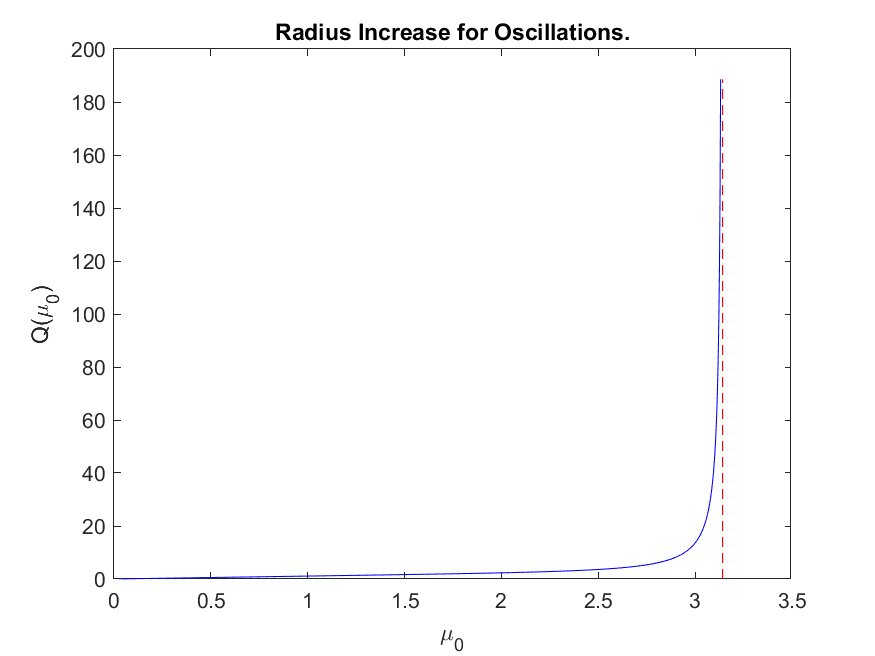
\includegraphics[width=0.8\textwidth]{images/Qmu.png}
    \caption{The plot of \(Q(\mu_0)\).}
    \label{fig:acrobot-Q}
\end{figure}

\subsubsection*{Energy Gain on \(\mathcal{O}_1\)}

The Poincar\'{e} map \(P_\mathcal{O}\) allows us understand the evolution of
\(\hat{\mu}(\alpha,\mu_0,I)\) by studying the evolution of the discrete time
system
\begin{equation}\label{eqn:muhat-discrete}
        \mu_{n+1} := P_\mathcal{O}(\mu_n) 
        = \mu_n + I K Q(\mu_n) + R(\pi,\mu_n,I)
        ,
\end{equation}
with initial condition \(\mu_0\).
Here, \(\mu_n\) represents the distance along the
\(q_u\)-axis when an orbit of the constrained dynamics intersects the
\(q_u\)-axis for the \(n\)th time, assuming the orbit was initialized at
\((q_u,p_u) = (\mu_0,0)\).

Proving the constrained dynamics gain energy on \(\mathcal{O}_1\) is equivalent to
showing \(\mu_n\) eventually reaches \(\pi\).
That is, we want to find \(I^\star \in\, ]0, I_1]\) where, for all 
\(\delta > 0\) and \(\mu_0 \in ]0,\pi-\delta]\), there exists \(N > 0\) so that
for all \(n \geq N\), \(\mu_n \notin [0,\pi-\delta]\).

A sufficient conditions for this characterization is to prove that 
\(P_\mathcal{O}(\mu_0) \geq \mu_0 + \gamma\) for some \(\gamma > 0\).
We will perform our analysis in two sections.
First, we will show the origin is a repeller of ~\eqref{eqn:muhat-discrete}.
This implies that orbits near the origin flow away from it.
Then, we will use the sufficient condition above to guarantee all orbits reach
\(\mu = \pi\).

Linearizing ~\eqref{eqn:muhat-discrete} at \(\mu_0 = 0\) yields
\[
    P^\prime_\mathcal{O}(0) = 1 + I K Q^\prime(0) +
    R^\prime(\pi,0,I)
    ,
\]
where prime denotes differentiation with respect to \(\mu\).
If there is some value of \(I \in \,]0,I_1]\) for which this term is greater than
\(1\), then \(0\) is a repeller of the discrete time system.
To show such a value of \(I\) exists, we first compute 
\[
    Q^\prime(0) = \int \limits_0^\pi \pdiff{a}{\mu}(\sigma,0) d\sigma
    .
\]
Numerical computations reveal that 
\[
    \lim \limits_{\mu_0 \to 0^+}
    \pdiff{a}{\mu}(\alpha,\mu_0) 
    = -\frac{\sqrt{2}}{2} \left(11\sin(\alpha)^2 - 6\right)
    ,
\]
which means 
\[
    Q^\prime(0)  = \frac{\pi}{2\sqrt{2}} > 0
    .
\]
Since the remainder term \(R(\pi,0,I)\) is \(O(I^2)\), 
its partial derivative \(R^\prime(\pi,0,I)\) is also \(O(I^2)\).
Hence, it can be written in the form
\(I^2 \tilde{R}(I)\) where \(\tilde{R}(I)\) is smooth and
zero at \(I = 0\).
Thus, there exists \(I_2 \in \,]0,I_1]\) such that
\[
    I_2 K Q^\prime(0) + (I_2)^2 \tilde{R}(I) > 0
    .
\]
Hence,
\[
    P^\prime_\mathcal{O}(0) \geq 1 + IKQ^\prime(0) + I^2 \tilde{R}(I) 
    > 1
    ,
\] 
for all \(I \in \,]0, I_2]\).

We have shown \(0\) is a repeller of the discrete time system, which means
there exists some (unknown) \(\epsilon > 0\) where the interval
\(]0,\epsilon[\) is negatively invariant for ~\eqref{eqn:muhat-discrete}.
What's more, all solutions starting in this interval will flow towards the value
\(\mu = \epsilon\).

To complete the proof, recall that \(R(\pi,\mu_0,I)\) is smooth in all its
parameters as well as being \(O(I^2)\).
It is therefore bounded below on the compact set \(\mu_0 \in [\epsilon,\pi]\)
by some value \(\underbar{R}(I)\). 
Theorem \ref{thm:khalil-perturbation} asserts that there exists some
\(I_3 > 0\) and \(r > 0\) so that, for all \(I \in [-I_3, I_3]\),
\[
    R(\pi,\mu_0,I) \geq \underbar{R}(I) > -I^2 r
    .
\]
Note that we can assume \(I_3 \leq I_2\) without loss of generality.
Furthermore, \(Q(\mu_0)\) is a strictly increasing function, so
for \(\mu_0 \in [\epsilon,\pi[\),
\[
    P_\mathcal{O}(\mu_0) > \mu_0 + I K Q(\epsilon) - I^2 r
    .
\]
Picking a small \(\gamma > 0\) and choosing 
\(I^\star \in\, ]0, I_3]\) so that
\[
    I^\star K Q(\epsilon) - (I^\star)^2 r \geq \gamma > 0
    ,
\]
means that \( P_\mathcal{O}(\mu_0) \geq \mu_0 + \gamma\)
for all \(\mu_0 \in [\epsilon,\pi[\).

Looking at ~\eqref{eqn:muhat-discrete} we find that
\(\mu_{n+1} \geq \mu_n + \gamma\). 
This implies that all solutions of the discrete time system will flow towards
\(\mu = \pi\).

We conclude that, for all \(m\), \(g\), \(l\), \(\bar{q}_a\), 
there exists \(I > 0\) small enough that the constraint 
~\eqref{eqn:acrobot-constraint} is injecting energy on \(\mathcal{O}_1\).

By the same arguments presented in this section, the Poincar\'{e} section
satisfies \(P_\mathcal{O}(\mu_0) \leq \mu_0 - \gamma\) when \(I < 0\). 
In this case, the constraint dissipates energy on \(\mathcal{O}_1\).

\subsubsection*{Energy Gain on \(\bar{\mathcal{O}}_1\)}
Before moving on to the rotation analysis, we must first confirm that any
acrobot constrained by ~\eqref{eqn:acrobot-constraint} will eventually start
rotating.
The definition of energy gain states that all orbits initialized in
\(\mathcal{O}_1\) will escape compact subsets of \(\mathcal{O}_1\) in finite time. 
This is not enough to prove that all orbits will escape the boundary of
\(\mathcal{O}_1\). 

Indeed, let \(E_\pi\) be the level set with energy \(E(\pi,0)\), 
which forms the boundary of \(\mathcal{O}_1\). 
Define \(\bar{\mathcal{O}}_1 = \mathcal{O}_1 \cup E_\pi\) to be the closure of
\(\mathcal{O}_1\).
An orbit of the acrobot will only begin rotating if it escapes
\(\bar{\mathcal{O}}_1\) by crossing through \(E_\pi\), and eventually remains
outside this set.
It is possible for orbits starting in \(\mathcal{O}_1\) to always approach
\(E_\pi\) without ever crossing into the rotation zone.
We will prove this does not happen in general.

To begin, let us analyze the upright equilibrium.
Taking the Jacobian of the constrained dynamics
~\eqref{eqn:acrobot-constrained-dynamics} at \((q_u,p_u) = (\pi,0)\) yields
\[
    J = \begin{bmatrix}
        -\frac{6mgl\bar{q}_aI}{5} & \frac{1 - 2m^2gl^3\bar{q}_a^2 I^2}{5ml^2} \\
        3mgl & mgl\bar{q}_aI
    \end{bmatrix}
    ,
\]
which has characteristic polynomial
\[
    \det\left(\lambda \Id{2} - J\right)
    = \lambda^2 + \frac{mgl\bar{q}_a I}{5} \lambda - 3g
    .
\]
By Descartes' rule of signs, this polynomial has one root with positive real
part. 
The equilibrium \((\pi,0)\) is therefore unstable, so the stable manifold \(\Pi^+\) of
initial conditions converging to \((\pi,0)\) is one-dimensional, and hence is
of measure zero in \(\SxR\).

Using \(x(t) := (q_u(t),p_u(t))\) as shorthand, let
\(x(0) \in \mathcal{O}_1\) be a nonzero initial condition of the acrobot.
Suppose by way of contradiction that the orbit \(x(\R)\) is confined within 
\(\bar{\mathcal{O}}_1\), and does not exit through \(E_\pi\) into the rotation
zone.
Since \(\bar{\mathcal{O}}_1\) is compact, the Birkhoff Theorem \cite{birkhoff}
implies:
\begin{itemize}
    \item The positive limit set \(L_+\) of \(x(t)\) is non-empty, compact, and
        invariant.
    \item The solution \(x(t)\) asymptotically tends to \(L_+\).
\end{itemize}
Since the acrobot gains energy on \(\mathcal{O}_1\), the positive limit set of
\(x(t)\) must be the largest invariant subset of \(E_\pi\). 
From our discussion on pseudo-polar coordinates (in particular the extension
~\eqref{eqn:alpha-dot-boundary} of \(\dot{\alpha}\) to \(\bar{\mathcal{O}}_1\)),
we know that \(\dot{\alpha} \geq 0\) on \(E_\pi\), with equality if and only if 
\(\alpha \in \{0,\pi\}\).
There are two possibilities: either \(E_\pi\) itself is invariant, or the
largest invariant subset of \(E_\pi\) is \(\{(\pi,0)\}\).
To rule out the first possibility, take the derivative of \(E(q_u,p_u)\) at the
\(p_u\)-axis to get
\[
    \dot{E}(0,p_u) = -\frac{g}{5l} \sin(q_a)p_u
    .
\]
This is non-zero everywhere except at the origin, which means it is non-zero on
\(E_\pi\). 
This means \(E_\pi\) is not invariant, so the positive limit set of \(x(t)\)
must be the set \(\{(\pi,0)\}\).
Hence, \(x(t)\) converges to \((\pi,0)\), which means \(x(0) \in \Pi^+\).
Since we know that \(\Pi^+\) is a set of measure zero in \(\SxR\), almost every
orbit initialized in \(\mathcal{O}_1\) must escape through the boundary
\(E_\pi\) into the rotation domain.

Escaping once into the rotation domain does not guarantee the acrobot
orbit will never return to \(\mathcal{O}_1\).
Indeed, the orbit could escape through \(E_\pi\) and return to \(\mathcal{O}_1\)
several times.
However, almost every orbit must eventually remain outside the closure of 
\(\mathcal{O}_1\). 
If not, the positive limit set would once again be
\(E_\pi\); by the same argument as above, that orbit would be in \(\Pi^+\).

We conclude that all orbits beginning in \(\mathcal{O}_1\) will, in finite time,
escape the closure of \(\mathcal{O}_1\) and remain in the rotation domain
forever after.

\subsubsection*{Summary}

We have proven the first part of Theorem \ref{thm:acrobot-energy-stabilization},
which claims there exists a control value \(I^\star > 0\) such that, for 
\(I \in \, ]0,I^\star]\), ~\eqref{eqn:acrobot-constraint} injects energy into
the acrobot on \(\mathcal{O}_1\).
Enough energy is injected that orbits will exit the closure of \(\mathcal{O}_1\)
and enter the rotation domain.

Here is a summary of the proof:
\begin{enumerate}
    \item We found pseudo-polar coordinates \((\alpha,\mu)\) adapted to level
        sets of the nominal pendulum's mechanical energy on \(\mathcal{O}_1\),
        where \(\alpha \in \Sone\) is a pseudo-angle and \(\mu \in \, ]0,\pi[\)
        is a pseudo-radius.
    \item We showed there exists a value \(I_1\) small enough where 
        \(\dot{\alpha} > 0\) everywhere on \(\mathcal{O}_1\).
    \item Using \(\alpha\) as a time variable, we found the time-scaled
        pseudo-radius \(\hat{\mu}\) and expanded it into
        ~\eqref{eqn:acrobot-muhat-approx} using perturbation theory.
    \item Taking this expanded solution, we defined and expanded the
        Poincar\'{e} map \(P_\mathcal{O}\) to analyze the discrete-time system
        ~\eqref{eqn:muhat-discrete}.
    \item We found a value \(I_2 \leq I_1\) making the origin a repeller of 
        ~\eqref{eqn:muhat-discrete}, and a value \(I_3 \leq I_2\) which drives
        \(\mu_n\) towards \(\mu = \pi\).
    \item We showed that the upright equilibrium \((\pi,0)\) is unstable, and
        used this fact to prove that almost every orbit crosses through
        \(E_\pi\), thereby exiting the closure of \(\mathcal{O}_1\) in finite
        time.
\end{enumerate}
Choosing \(I \in \,]0,I_3]\) guarantees energy injection on
\(\mathcal{O}_1\) because all orbits approach the pseudo-radius \(\mu = \pi\).
In fact, almost all orbits escape \(\bar{\mathcal{O}}_1\).
Likewise, choosing \(I \in [-I_3,0[\) guarantees energy dissipation on
\(\mathcal{O}_1\).

% Empty proof environment to put QED square on the right of the page
\begin{proof}[\unskip\nopunct]
\end{proof}

\subsection{Perturbation Analysis for Rotations}
Figure \ref{fig:pendulum-level-sets} reminds us that rotations of the 
nominal pendulum obtained by setting \(I = 0\) look like open curves on some
rotation domain \(\mathcal{R} \subset \SxR\), where
\[
    \mathcal{R} := \left\{ (q_u,p_u) \in \SxR \mid E(q_u,p_u) > E(\pi,0)\right\}
    .
\]
Performing a similar process to what we did for oscillations,
we wish to find a new set of coordinates \((\beta,\rho)\)
where the pseudo-radius \(\rho \in \mathbb{R}\) remains constant on level sets
of \(E\) and the pseudo-angle \(\beta \in \Sone\) is always increasing on
\(\mathcal{R}\).

\subsubsection*{Pseudo-Polar Coordinates}

In the oscillation region \(\mathcal{O}_1\) we showed that the energy of the
nominal pendulum \eqref{eqn:acrobot-nominal-dynamics} is uniquely determined by
an orbit's intersection point \(\mu\) with the \(q_u\)-axis.
Likewise, on \(\mathcal{R}\) the energy is determined by the orbit's intersection
point \(\rho\) with the \(p_u\)-axis, as in Figure \ref{fig:rho-intersection}.

\begin{figure}
    \centering
    \includestandalone[]{images/rho_intersection}
    \caption{The domain \(\mathcal{R}\) (blue) where a pendulum rotates. The
        pseudo-radius \(\rho\) corresponds to the intersection of an orbit of
        rotation with the \(p_u\)-axis. The pseudo-angle \(\beta\) selects a
        point on the rotation.}
    \label{fig:rho-intersection}
\end{figure}

Note that the boundary of \(\mathcal{R}\) intersects the \(p_u\) axis when 
\(p_u^2 = 60m^2 g l^3\). 
This boundary is the homoclinic orbit for the
upright equilibrium of the pendulum, which is the level set with energy
\(E(\pi,0)\).
Hence, we must have \(\rho > \sqrt{60 m^2 g l^3}\), if a
rotation has momentum \(p_u > 0\), 
and \(\rho < -\sqrt{60 m^2 g l^3}\) if it has momentum \(p_u < 0\).
The energy level set associated with \(\rho\) is 
\[
    \left\{(q_u,p_u) \in \SxR \mid E(q_u,p_u) = \frac{\rho^2}{10ml^2}\right\}
    ,
\]
which gives the relationship
\begin{equation}\label{eqn:rotation-pu2}
    \frac{p_u^2}{10m l^2} + 3mgl(1 - c_u) = \frac{\rho^2}{10 ml^2}
    .
\end{equation}
On this level set, \(q_u\) takes all values on \(\Sone\), so our angle of
rotation is uniquely parameterized by \(\beta = q_u\).
Since \(\rho\) does not change sign along the rotation, we have the smooth
relationship
\begin{align}\label{eqn:rotation-Tinv}
    q_u &= \beta
    , \\
    p_u &= \sign{\rho}\sqrt{\rho^2 - 30 m^2 g l^3\left(1 - c_\beta \right)}
    .
\end{align}

Inverting this relationship gives our pseudo-polar coordinates
\begin{align}\label{eqn:rotation-T}
    \beta &= q_u
    , \\
    \rho &= \sign{p_u}\sqrt{p_u^2 + 30 m^2 g l^3 \left(1 - c_u \right)}
    .
\end{align}

Computing the acrobot's constrained dynamics in \((\beta,\rho)\)-coordinates and
setting \(I = 0\) yields the dynamics of the nominal pendulum.
MATLAB evaluates those dynamics as
\begin{align}
    \label{eqn:acrobot-rot-alpha-dot-nom}
    \dot{\beta} &=  \sign{\rho} 
    \frac{\sqrt{\rho^2 - 30m^2gl^3(1 - c_\beta)}}{5ml^2}
    , \\
    \label{eqn:acrobot-rot-mu-dot-nom}
    \dot{\rho} &= 0
    .
\end{align}
As expected, \(\dot{\beta}\) does not change sign on \(\mathcal{R}\) because the
orbits always flow clockwise.
If \(\rho > 0\), the rotation curve goes from \(\beta = -\pi\) to 
\(\beta = \pi\); 
if \(\rho < 0\), it goes from \(\beta = \pi\) to \(\beta = -\pi\).
By continuity of ~\eqref{eqn:rotation-T}, there exists \(I_1 > 0\) small enough
that \(\dot{\beta}\) is non-zero and does not change sign on \(\mathcal{R}\) for
all \(I \in [-I_1,I_1]\).

\subsubsection*{Time Scaling}

Using \(\beta\) as our new time variable (via a time reparameterization
\(t = t(\beta)\)) produces the time-scaled pseudo-radius
\(\hat{\rho}(\beta) := \rho(t(\beta))\).
This reduces the system \((\dot{\beta},\dot{\rho})\) into the scalar time-varying
ODE
\begin{equation}\label{eqn:rhohat-dot}
    \begin{cases}
        \diff{\hat{\rho}}{\beta} = \frac{\dot{\rho}}{\dot{\beta}}
        , \\
        \hat{\rho}(0) = \rho_0
        .
    \end{cases}
\end{equation}

\subsubsection*{Perturbation Analysis of the Time Scaled System}

In the spirit of perturbation analysis, we expand the time-scaled system 
\(\hat{\rho}(\beta,\rho_0,I)\). 
From ~\eqref{eqn:khalil-perturbation-nominal} we know the nominal system at
\(I = 0\) is
\[
    \begin{cases} 
        \diff{\hat{\rho}_0}{\beta} = 0
        , \\
        \hat{\rho}_0(0) = \rho_0
        ,
    \end{cases}
\]
which has solution \(\hat{\rho}_0(\beta,\rho_0) \equiv \rho_0\).

We take a first-order Taylor approximation of \(\hat{\rho}(\beta,\rho_0,I)\)
around \(\hat{\rho}_0(\beta,\rho_0)\) to get
\begin{equation}\label{eqn:acrobot-rhohat-approx}
    \hat{\rho}(\beta,\rho_0,I) = \hat{\rho}_0(\beta,\rho_0) +
    I\hat{\rho}_1(\beta,\rho_0) + R(\beta,\rho_0,I)
    ,
\end{equation}
where \(R(\beta,\rho_0,I)\) is smooth and \(O(I^2)\).

Using MATLAB's symbolic toolbox and 
~\eqref{eqn:khalil-perturbation-firstorder}, 
we discover that \(\hat{\rho}_1(\beta,\rho_0)\) is the solution to the linear
time-varying scalar ODE
\begin{equation}\label{eqn:acrobot-rho1-dot}
  \begin{cases}
      \diff{\hat{\rho}_1}{\beta} =
    \frac{5m^2 g l^3 \bar{q}_a \left(
        m^2gl^3\left(18s_\beta^2 + 30c_\beta(1 - c_\beta)\right)
        - c_\beta\rho_0^2
    \right)}{
    |\rho_0|\sqrt{\rho_0^2 - 30m^2gl^3(1 - c_\beta)}
    }
    =: b(\beta,\rho_0)
     , \\
     \hat{\rho}_1(0) = 0
     ,
 \end{cases}
\end{equation}
whose solution is
\[
    \hat{\rho}_1(\beta,\rho_0) = \int \limits_0^\beta b(\sigma,\rho_0)d\sigma
    .
\]

\subsubsection*{Poincar\'{e} Analysis}

Suppose we initialize the acrobot at \((\beta,\rho) = (0,\rho_0)\).
One full rotation amounts to \(\beta\) traversing \(2\pi\) rad in a clockwise
direction; that is, when \(\beta\) goes from \(0\) to \(\sign{\rho_0}2\pi\).
Since \(\dot{\beta}\) does not change sign on \(\mathcal{R}\),
there is a well-defined Poincar\'{e} map describing how the pseudo-radius
\(\rho\) changes each time the orbit \((q(t),p(t))\) hits the \(p_u\) axis, \ie
every time \(\beta\) changes by \(2\pi\).
We define this Poincar\'{e} map as
\[
    P_\mathcal{R}(\rho_0) := \hat{\rho}\left(\sign{\rho_0}2\pi,\rho_0,I\right)
    ,
\]
which expands into
\[
    P_\mathcal{R}(\rho_0) = \rho_0 + I \hat{\rho}_1(\sign{\rho_0}2\pi, \rho_0)
    + R(\sign{\rho_0}2\pi,\rho_0,I)
    .
\]

Let us pause here for a moment to remember what we are trying to accomplish.
The second part of Theorem \ref{thm:acrobot-energy-stabilization} states that,
under suitable conditions on the integral of \(b(\beta,\rho_0)\), 
the acrobot will gain energy on 
\[
    \mathcal{O}_2(\bar{\rho}) := \left\{ (q_u,p_u) \in \SxR
    \mid E(q_u,p_u) < E(0,\bar{\rho}) \right\}
    ,
\]
for some \(\bar{\rho} > \sqrt{60m^2gl^3}\).
Recall from Chapter \ref{sec:acrobot-proof-o1} that any acrobot initialized in
\(\mathcal{O}_1\) will eventually remain in the rotation region \(\mathcal{R}\).
What remains, then, is to prove that the acrobot's orbits will also gain
energy on
\[
    \mathcal{R}_{\bar{\rho}} := \mathcal{R} \cap \mathcal{O}_2(\bar{\rho})
    .
\]
This can be proven by analyzing the Poincar\'{e} map \(P_\mathcal{R}(\rho_0)\).
Looking at Figure \ref{fig:acrobot-rhobar-regions}, it is clear that
\(P_\mathcal{R}\) has the domain
\[
    D := \left[-\bar{\rho},-\sqrt{60m^2gl^3}\right[ \, 
    \cup \, 
    \left]\sqrt{60m^2gl^3},\bar{\rho}\right]
    ,
\]
which is the intersection of \(\mathcal{R}_{\bar{\rho}}\) with the \(p_u\)-axis.
We label the part of \(D\) contained in the negative \(p_u\)-axis as
\[
    D^- :=\left[-\bar{\rho},-\sqrt{60m^2gl^3}\right[
    ,
\]
and the part contained in the positive \(p_u\)-axis as
\[
    D^+ := \left]\sqrt{60m^2gl^3},\bar{\rho}\right]
    ,
\]
so that \(D = D^- \cup D^+\).
If \(P_\mathcal{R}(\rho_0)\) is always further from the origin than 
\(\rho_0\) (\ie it is ``expanding" on \(D\)), the acrobot will be gaining energy
on \(\mathcal{O}_2(\bar{\rho})\).

\begin{figure}
    \centering
    \includestandalone[width=0.5\textwidth]{images/acrobot_rhobar_regions}
    \caption{The region \(\mathcal{R}_{\bar{\rho}}\) of rotations in
        \(\mathcal{O}_2(\bar{\rho})\) is coloured
        in blue, while the domain \(D = D^- \cup D^+\) of the Poincar\'{e} map 
        is coloured in red.}
    \label{fig:acrobot-rhobar-regions}
\end{figure}

Mirroring the Poincar\'{e} analysis for oscillations, let us find a
function \(S(\rho_0)\) which is positive on \(D\).
This will be the rotational analogue to \(Q(\mu_0)\) from
~\eqref{eqn:acrobot-Qmu}.

Notice that the function \(b(\beta,\rho_0)\) is even and
\(2\pi\)-periodic in \(\beta\), which implies that
\begin{align*}
    \hat{\rho}_1(\sign{\rho_0}2\pi, \rho_0) &=
    \int \limits_0^{\sign{\rho_0}2\pi} b(\sigma,\rho_0)d\sigma
    , \\
     &=\sign{\rho_0}\int\limits_0^{2\pi}b(\sigma,\rho_0)d\sigma
     , \\
     &= \sign{\rho_0} \hat{\rho}_1(2\pi,\rho_0)
     .
\end{align*}
Defining \(S(\rho_0) := \hat{\rho}_1(2\pi,\rho_0)\),
the Poincar\'{e} map becomes
\begin{equation}\label{eqn:acrobot-poincare-r}
    P_\mathcal{R}(\rho_0) = \rho_0 + I\sign{\rho_0}S(\rho_0) 
    + R(\sign{\rho_0}2\pi,\rho_0,I)
    .
\end{equation}

Proving expansion of \(P_\mathcal{R}(\rho_0)\) becomes easier if
\(S(\rho_0)\) is positive on \(D\).
Recall the assumption that there exists
\(\epsilon > 0\) where \(S(\rho_0) \geq \epsilon\) for all 
\(\rho_0 \in D^+\).
Since \(b(\beta,\rho_0)\) is even in \(\rho_0\),
its integral \(S(\rho_0)\) is also even in \(\rho_0\),
which means \(S(\rho_0) \geq \epsilon\) for every \(\rho_0 \in D\).

\subsubsection*{Energy Gain on \(\mathcal{O}_2(\bar{\rho})\)}
The Poincar\'{e} section \(P_\mathcal{R}\) allows us understand the evolution of
\(\hat{\rho}(\beta,\rho_0,I)\) by studying the evolution of the discrete time
ODE
\begin{equation}\label{eqn:rhohat-discrete}
    \rho_{n+1} := P_\mathcal{R}(\rho_n) 
    = \rho_n + I\sign{\rho_n}S(\rho_n) + 
        R(\sign{\rho_n}2\pi,\rho_n,I)
    .
\end{equation}
Here, \(\rho_n\) represents the distance along the
\(p_u\)-axis when an orbit of the constrained dynamics intersects the
\(p_u\)-axis for the \(n^\text{th}\) time, assuming the orbit was initialized at
\((q_u,p_u) = (0,\rho_0)\).

To prove energy gain on \(\mathcal{R}_{\bar{\rho}}\), it is
enough to prove that \(\abs{\rho_n}\) eventually reaches \(\bar{\rho}\).
This is true if there exists some \(\gamma > 0\)
whereby \(\abs{P_\mathcal{R}(\rho_0)} \geq \abs{\rho_0} + \gamma\) for all 
\(\rho_0 \in D\)

We begin with \(\rho_0 \in D^+\).
Recall that \(R(\beta,\rho_0,I)\) is \(O(I^2)\) and smooth in all
its parameters.
Therefore, it is bounded below on the compact set
\(\rho_0 \in \left[\sqrt{60m^2gl^3},\bar{\rho}\right]\) by some value
\(\underbar{R}(I)\).
Theorem \ref{thm:khalil-perturbation} asserts that there exists some 
\(I_2 > 0\) and \(r > 0\) so that, for all \(I \in [-I_2,I_2]\),
\[
    R(2\pi,\rho_0,I) \geq \underbar{R}(I) > -I^2r
    .
\]
Since \(S(\rho_0) \geq \epsilon\), we find that
\[
    P_\mathcal{R}(\rho_0) > \rho_0 + I\epsilon -I^2r
    ,
\]
for all \(\rho_0 \in D^+\).
Choosing \(I_3 \in \,]0,I_2]\) so that
\[
    I_3\epsilon - (I_3)^2 r \geq \gamma
    ,
\] 
makes \(P_\mathcal{R}(\rho_0) \geq \rho_0 + \gamma\) for all 
\(\rho_0 \in D^+\).

Now take \(\rho_0 \in D^-\), where we wish to show that 
\(P_\mathcal{R}(\rho_0) \leq \rho_0 - \gamma\).
The remainder \(R(\beta,\rho_0,I)\) is bounded above on the compact set 
\(\rho_0 \in \left[-\bar{\rho},-\sqrt{60m^2gl^3}\right]\), and 
Theorem \ref{thm:khalil-perturbation} asserts that there exists some 
\(I_4 > 0\) and \(r^\prime > 0\) so that, for all \(I \in [-I_4,I_4]\), 
\[
    R(-2\pi,\rho_0,I) < I^2 r^\prime
    .
\]
Hence,
\begin{align*}
    P_\mathcal{R}(\rho_0) < \rho_0 - I\epsilon + I^2r^\prime
    .
\end{align*}
Choosing \(I_5 \in ]0,I_4]\) so that 
\[
    I_5 \epsilon - (I_5)^2r^\prime \geq \gamma
    ,
\] 
makes \(P_\mathcal{R}(\rho_0) \leq \rho_0 - \gamma\) for all 
\(\rho_0 \in D^-\).

To connect the two subregions of \(D\) together, choose
\(I^\star \in\, ]0,\min\left\{I_3,I_5\right\}]\).
Then \(\abs{P_\mathcal{R}(\rho_0)} \geq \abs{\rho_0} + \gamma\) for all
\(\rho_0 \in D\), so the constrained dynamics are gaining energy on 
\(\mathcal{R}_{\bar{\rho}}\).

By the same arguments presented in this section, the Poincar\'{e} section
satisfies 
\(\abs{P_\mathcal{R}(\rho_0)} \leq \abs{\rho_0} - \gamma\)
when \(I < 0\).

\subsubsection*{Conclusion}
We have proven the second part of Theorem
\ref{thm:acrobot-energy-stabilization}: if the acrobot satisfies the assumptions
on \(S(\rho_0)\), there exists \(I > 0\) small enough that the constraint
~\eqref{eqn:acrobot-constraint} injects energy into the acrobot on
\(\mathcal{O}_2(\bar{\rho})\).

Here is a summary of the proof:
\begin{enumerate}
    \item We found pseudo-polar coordinates \((\beta,\rho)\) adapted to level
        sets of the nominal pendulum's mechanical energy on \(\mathcal{R}\),
        where \(\beta \in \Sone\) is a pseudo-angle and
        \(\rho \in D\) is a pseudo-radius.
    \item We showed there exists a value \(I_1\) small enough where
        \(\dot{\beta} > 0\) everywhere on \(\mathcal{R}\).
    \item Using \(\beta\) as a time variable, we found the evolution of the
        time-scaled pseudo-radius \(\hat{\rho}\) and expanded it into
        ~\eqref{eqn:acrobot-rhohat-approx} using perturbation theory.
    \item Taking this expanded solution, we defined and expanded the
        Poincar\'{e} map \(P_\mathcal{R}\) on the domain 
        \(D = D^- \cup D^+\) which shows how the acrobot's orbits behave on
        \(\mathcal{R}_{\bar{\rho}}\).
    \item Using the Poincar\'{e} map to analyze the discrete-time system
        ~\eqref{eqn:rhohat-discrete}, we found values \(I_2,I_4\) bounding the
        remainder term \(R(\beta,\rho_0,I)\) on \(D^+\) and \(D^-\)
        (respectively), then found values \(I_3, I_5\) which drive all orbits of
        ~\eqref{eqn:rhohat-discrete} towards \(\abs{\rho} = \bar{\rho}\).
\end{enumerate}
Recall from Chapter \ref{sec:acrobot-proof-o1} that there exists \(I^\star > 0\)
making orbits escape \(\bar{\mathcal{O}}_1\) into 
\(\mathcal{R}\). 
Choosing \(I \in \,]0,\min\{I_3,I_5,I^\star\}]\)
guarantees energy injection on \(\mathcal{O}_2(\bar{\rho})\).
Likewise, choosing \(I \in [-\min\{I_3,I_5,I^\star\},0[\) guarantees energy
dissipation on \(\mathcal{O}_2(\bar{\rho})\).

This analysis, together with that of Chapter \ref{sec:acrobot-proof-o1},
completes the proof of Theorem \ref{thm:acrobot-energy-stabilization}.

% Draw the proof square only
\begin{proof}[\unskip\nopunct]
\end{proof}

\section{Experimental Results}
In this section, we test our VNHC on the physical acrobot built by
Xingbo Wang \cite{xingbo_thesis} (Figure \ref{fig:xingbo-acrobot}).
This acrobot is not simple, that is, the torso and leg rods have unequal mass
and differ in length. 
Furthermore, the centers of mass are not located at the tip of each rod.
These experiments will therefore test whether VNHCs are robust to model
mismatch, since our VNHC is only proven to inject energy on simple acrobots.
As we will see, our VNHC does inject energy on the general acrobot model.

\begin{figure}
    \centering
    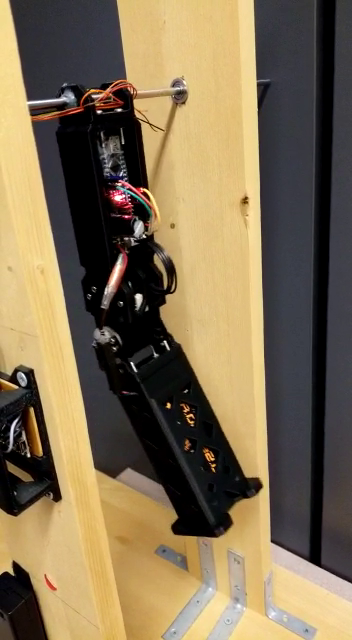
\includegraphics[width=0.5\linewidth]{images/xingbo_acrobot.png}
    \caption{The acrobot built by Wang \cite{xingbo_thesis}.}
    \label{fig:xingbo-acrobot}
\end{figure}

Wang's acrobot  has inertia matrix as in ~\eqref{eqn:general-acrobot-inertia}
and potential function as in ~\eqref{eqn:general-acrobot-potential}.
The physical parameters are written explicitly in Table
\ref{tab:acrobot-parameters}.

\begin{table}
    \centering
    \caption{Physical parameters for the real acrobot, as measured by
    \citet{xingbo_thesis}.}
    \label{tab:acrobot-parameters}
    \begin{tabular}{ccccccccc}
        \toprule
        $m_u$ & $m_a$ & $l_u$ & $l_a$ & $l_{c_u}$ & $l_{c_a}$ & $J_u$ & $J_a$ & $g$ \\
        \midrule
        0.2112 & 0.1979 & % mass
        0.148 & 0.145 & % total length
        0.073 & 0.083 & % COM distance
        0.00129 & 0.00075 & % moment of inertia
        9.81 \\ % gravity
        \bottomrule
    \end{tabular}
\end{table}

This acrobot's actuator is a servo motor with a built-in PID controller, so we
can set \(q_a = \arctan\left(I p_u\right)\) directly without needing to solve
for the VNHC's torque input \(\tau\).
The control parameter \(I\) needs to be small, but it also needs to be large
enough to overcome friction in the servo motor.
Since the acrobot's mass and length values are small, its momentum is
also small.
Through various experiments, we determined that \(I = 10\) is sufficient to
ensure the actuator can fully rotate in its allowable range
\(q_a \in \left[ -\frac{\pi}{2}, \frac{\pi}{2}\right]\).

\subsection{Simulations}

To compute the energy of the nominal pendulum, we evaluate the system at the
VNHC \(q_a = 0\), which yields
\[
    E(q_u,p_u) \approx 396.5501 p_u^2 + 0.5997(1 - \cos(q_u))
    .
\]
Hence, the level set of \(E_\pi\) of the energy \(E(\pi,0)\) is parameterized by
\begin{align*}
    p_u &\approx \pm \sqrt{\frac{1.1994}{793.1001}(1 + \cos(q_u))}
    ,
\end{align*}
for each \(q_u \in ]-\pi,\pi]\).

\begin{figure}[ht]
    \centering
    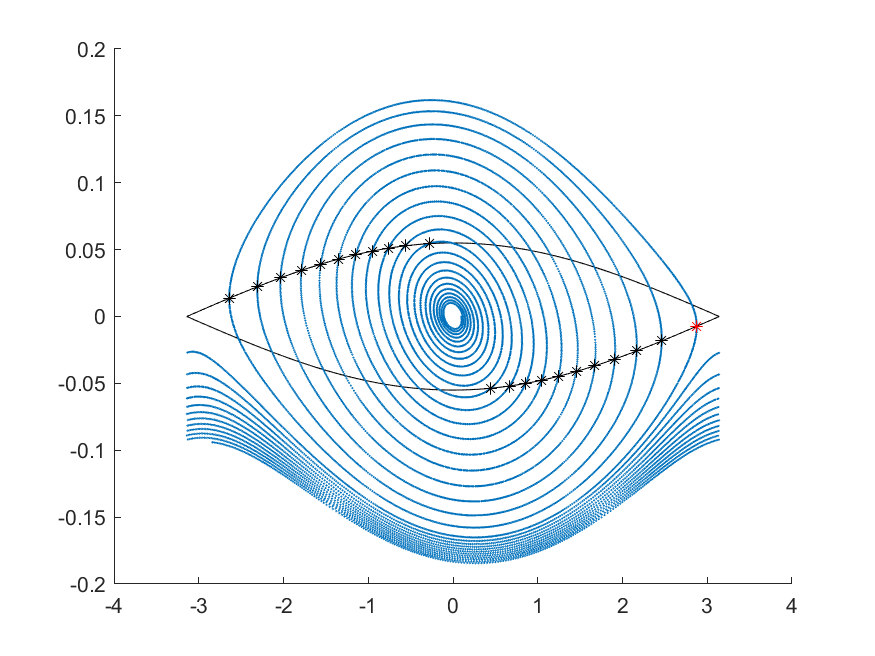
\includegraphics[width=0.8\linewidth]{images/acrobot_orbit.png}
    \caption{A simulation of the acrobot from \cite{xingbo_thesis}.}
    \label{fig:acrobot-orbit}
\end{figure}

We initialize the simulation for this acrobot at 
\((q_u,p_u) = \left(\frac{\pi}{32},0 \right)\) and plot the resulting orbit in 
Figure \ref{fig:acrobot-orbit}.
The nominal energy level set \(E_\pi\) is outlined in black. 
Because this acrobot is not simple, \(E_\pi\) is not the boundary between
rotations and oscillations.
The oscillation domain is actually much larger: orbits rotate once they hit the
\(p_u\)-axis at \(\abs{p_u} \approx 0.15\), while \(E_\pi\) intersects the
\(p_u\)-axis at \(\abs{p_u} \approx 0.055\).
Despite this, we see that eventually the acrobot remains outside \(E_\pi\).
The points where the orbit exits \(E_\pi\) are highlighted with black stars,
with the final departure highlighted in red.
At this final departure, the acrobot begins rotating and continues to gain
energy over time.

To verify that the acrobot will consistently begin rotating, we use a Monte
Carlo method \cite{montecarlo} to simulate this
acrobot \(1000\) times.
At each iteration, we initialize the acrobot randomly inside the sublevel set
\[
    \left\{(q_u,p_u) \in \SxR \mid
    E(q_u,p_u) \leq E\left(\frac{\pi}{32},0\right)\right\}
    ,
\] 
and measure how long it takes the acrobot to begin rotating.
The results are plotted in Figure \ref{fig:acrobot-mc}.
The acrobot always rotates within 10--35 seconds.

\begin{figure}
    \centering
    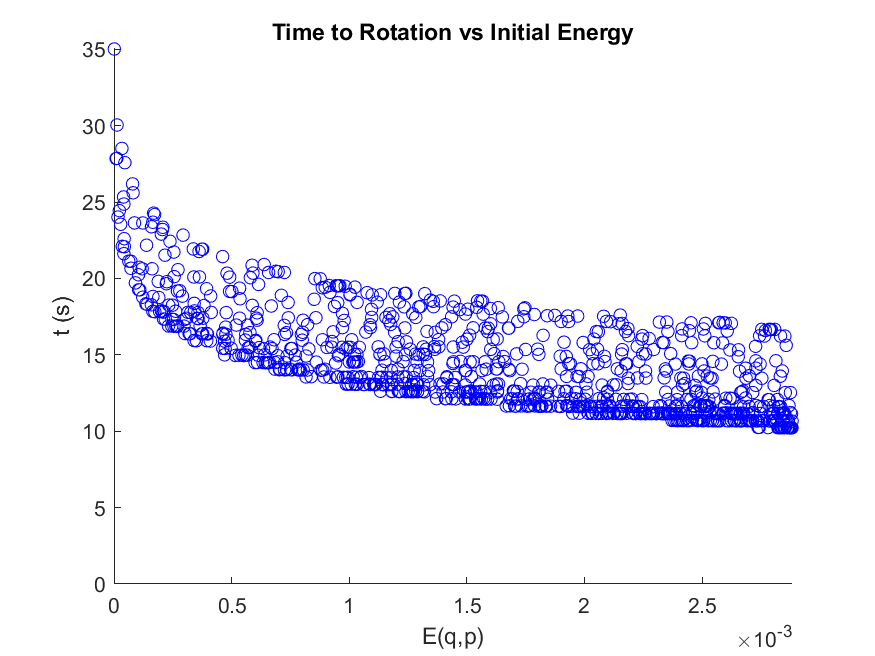
\includegraphics[width=0.8\textwidth]{images/acrobot_mc.png}
    \caption{Monte Carlo simulation results for the acrobot from
    \cite{xingbo_thesis}.}
    \label{fig:acrobot-mc}
\end{figure}

\subsection{Physical Experiments}
To complete this chapter, we perform four experiments with the physical
acrobot:
\begin{enumerate}
    \item An undisturbed test to validate that the acrobot reaches rotations.
    \item A test where we stop the acrobot once it has started rotating.
    \item A test where we push the acrobot in its direction of motion after it has
        started rotating.
    \item A test where we push the acrobot against its direction of motion.
\end{enumerate}

The acrobot has an encoder at the pivot which measures \(q_u\) and
\(\dot{q}_u\), and the servo provides a measurement of \(q_a\).
We estimate \(\dot{q}_a\) through sequential values of \(q_a\) and
compute \(p_u\) through \(p_u = e_1^T M(q) \dot{q}\).
The actuator value at iteration \(k \in \mathbb{Z}_{> 0}\) is assigned through
the equation
\[
    q_a^{k} = \arctan(I p_u^{k-1})
    .
\]

\subsubsection*{Test 1: No Disturbances}
For this test we initialize the acrobot at 
\((q_u,p_u) \approx \left(\frac{\pi}{8},0\right)\). 
The resulting orbit is shown in Figure \ref{fig:acrobot-unperturbed-orbit},
which is clearly gaining energy over time.

\begin{figure}[ht]
    \centering
    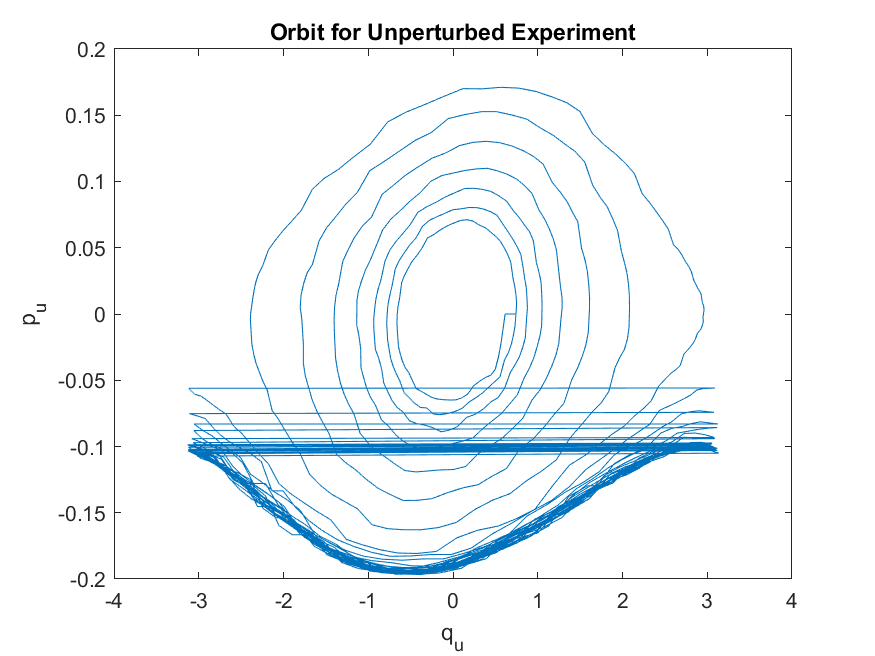
\includegraphics[width=0.5\linewidth]{images/acrobot_unperturbed_orbit.png}
    \caption{The orbit of the physical acrobot during an unperturbed test.}
    \label{fig:acrobot-unperturbed-orbit}
\end{figure}

\subsubsection*{Test 2: Stopping the Acrobot}
For this test we initialize the acrobot at 
\((q_u,p_u) \approx \left(\pi,0\right)\) and let it run for 15
seconds, then stop the acrobot as it reaches the bottom of its arc.
The resulting orbit is shown in Figure \ref{fig:acrobot-stopped-orbit}.
The blue curves correspond to the orbit before the disturbance, while the red
spiral shows that the acrobot begins oscillating after it is stopped.
Despite the disturbance, it gains energy and eventually starts rotating
again.

\begin{figure}[ht]
    \centering
    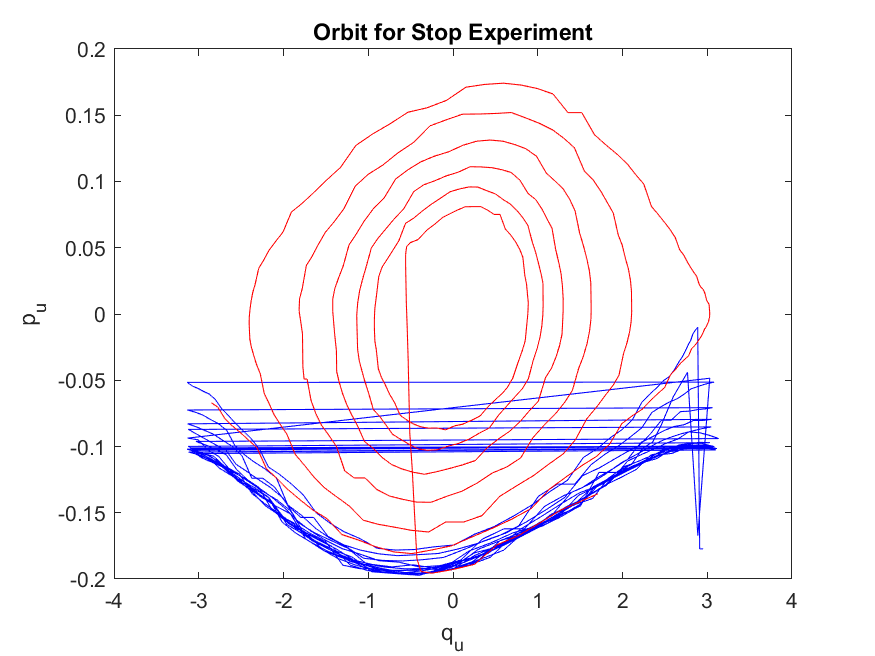
\includegraphics[width=0.5\linewidth]{images/acrobot_stopped_orbit.png}
    \caption{The orbit of the physical acrobot before (blue) and after (red) it
    is stopped.}
    \label{fig:acrobot-stopped-orbit}
\end{figure}

\subsubsection*{Test 3: Pushing the Acrobot Forwards}
To see how the acrobot responds when pushed in its direction of motion, we allow
the acrobot to rotate undisturbed for 15 seconds and then give it a push in its
direction of motion.
The orbit in Figure \ref{fig:acrobot-fpush-orbit} shows that the acrobot speeds
up to rotate with energy \(E(0,0.22)\), but then slows down until it reaches a
stable rotation with energy \(E(0,-0.195)\).

\begin{figure}[ht]
    \centering
    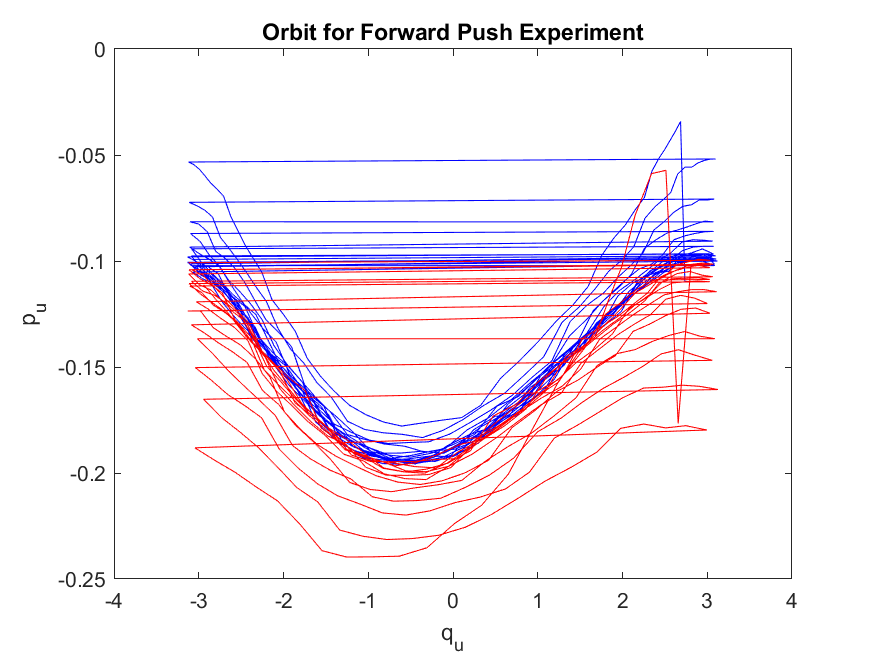
\includegraphics[width=0.5\textwidth]{images/acrobot_fpush_orbit.png}
    \caption{The orbit of the physical acrobot before (blue) and after (red) it
    is pushed in its current direction of motion.}
    \label{fig:acrobot-fpush-orbit}
\end{figure}

\subsubsection*{Test 4: Pushing the Acrobot Backwards}
In this final experiment, we test whether the acrobot can easily change
directions when pushed against its current direction of motion.
We again allow the acrobot to rotate undisturbed for 15 seconds, then push it
the opposite way.
The orbit in Figure \ref{fig:acrobot-rpush-orbit} demonstrates that the acrobot
responds by readily changing direction, and quickly achieves its maximum speed
with energy \(E(0,0.195)\).

\begin{figure}[ht]
    \centering
    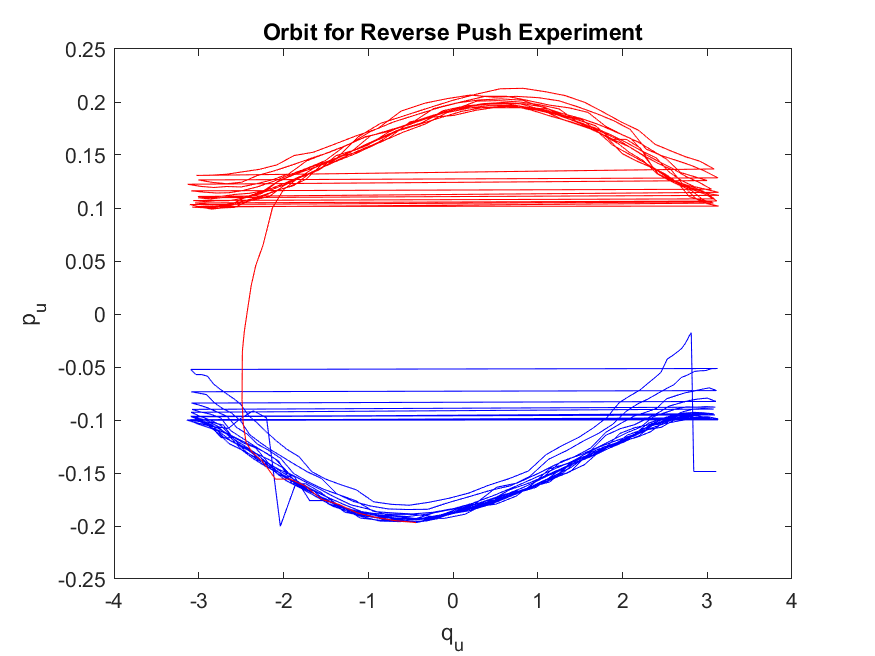
\includegraphics[width=0.5\textwidth]{images/acrobot_rpush_orbit.png}
    \caption{The orbit of the physical acrobot before (blue) and after (red) it
    is pushed against its current direction of motion.}
    \label{fig:acrobot-rpush-orbit}
\end{figure}

\subsection{Summary of Experimental Results}
The simulations and experiments in this section show that VNHCs are excellent
tools for injecting energy even in non-simple acrobots. 
Furthermore, the experimental results show that the energy gain is robust
against a variety of disturbances.
Finally, the two push tests suggest that Wang's acrobot constrained by our VNHC
will gain energy on \(\mathcal{O}_2(0.195)\).

%/========== /Acrobot ==========/%
% vim: set tw=80 ts=4 sw=4 sts=0 et ffs=unix :


% Concluding remarks and future work
%! TEX root = main.tex

%/========== Conclusion ==========/%

\chapter{Conclusion}\label{ch:conclusion}

This thesis has shown the utility of VNHCs as a means of injecting energy into
mechanical systems.
In Chapter \ref{ch:vnhcs} we developed the framework of VNHCs for underactuated
mechanical systems, with a focus on VNHCs for simply actuated Hamiltonian
systems.
We then applied this framework to two benchmark systems: the variable-length
pendulum and the acrobot.
In Chapter \ref{ch:vlp} we proved that a certain class of VNHCs will always
inject energy into the VLP, while in Chapter \ref{ch:acrobot} we designed a
constraint inspired by gymnastics and proved it injects energy into the
acrobot.
At the end of each chapter we performed simulations and experiments which
validated the theory and showed the utility of VNHCs. 
In the end, we demonstrated that virtual nonholonomic constraints are capable of
injecting and dissipating energy in a robust manner, all while producing
realistic biological motion.

\section{Limitations and Future Research}
Our VNHC framework relies on the following assumptions:
\begin{enumerate}
    \item The input matrix \(B(q) \equiv B \in \R^{n \times k}\) is constant and
        full rank.
    \item The input matrix has a left-annihilator 
        \(B^\perp \in \R^{(n-k)\times n}\). 
    \item The annihilator matrix \(B^\perp\) is right semi-orthogonal.
    \item The inertia matrix of the system satisfies 
        \(\nabla_{q_u}M(q) = \Zmat{n(n-k) \times n}\).
    \item On the constraint manifold \(\Gamma\), one can solve for \(q_a\) as a
        function of \((q_u,p_u)\).
\end{enumerate}
If any of these assumptions are not satisfied, one may not be able to find the
constrained dynamics in simply actuated coordinates, and the results of this
thesis may not hold.
In particular, the theoretical guarantees of this thesis do not apply to systems
with physical nonholonomic constraints (\eg friction), nor do they apply to vehicles
with wheels.

These limitations guide us to the following research directions. 
First, one might relax the assumptions on the input and inertia
matrices, thereby widening the class of systems to which VNHCs can be applied.
Second, one might forgo the assumption that \(q_a\) is solvable on the
constraint manifold; instead, one could borrow from the VHC literature
and parameterize the constraint manifold with a different set of
coordinates than \((q_u,p_u)\).
Third, one might consider more general mechanical systems with dynamics given by
\[
    \begin{cases}
        \dot{q} = \Minv(q) p
        , \\
        \dot{p} = -\pdmat - \nabla_q V(q) + Q_{nh}(q,p) + B(q)\tau
        ,
    \end{cases}
\]
where \(Q_{nh}(q,p) \in \R^n\) are terms corresponding to physical nonholonomic
constraints like friction.
Fourth, one can investigate a smoother method for energy stabilization, where
a VNHC is explicitly designed to inject energy below some energy level, and
dissipate energy above it.
For example, one might devise a mechanism for smoothly transferring
between VNHCs while maintaining certain safety requirements.

Finally, the proof of Theorem \ref{thm:acrobot-energy-stabilization} 
in Chapter \ref{sec:acrobot-proof} opens a door to the possibility of VNHC generation. 
One might search for suitable conditions on VNHCs where the Poincar\'{e}
sections for oscillations and rotations are increasing.
Then, one can extend Otsason's ``virtual constraint
generator" \cite{vcg} to generate regular VNHCs which satisfy
these energy injection/dissipation conditions.
In this way, one could automatically generate regular VNHCs which stabilize a
desired energy level.

%/========== /Conclusion ==========/%
% vim: set tw=80 ts=4 sw=4 sts=0 et ffs=unix :


%---------- Bibliography ----------%
%\newpage
% This adds a line for the Bibliography in the Table of Contents.
\addcontentsline{toc}{chapter}{Bibliography}
\printbibliography
\end{document}
%/========== /Main Document ==========/%

% vim: set tw=80 ts=4 sw=4 sts=0 et ffs=unix :
